%version of 04-09-20

\chapter{Sets and Their Algebras:
The Stem Cells of Mathematics}
\label{ch:sets-BA-logic}

\begin{quote}
``Les grands math\'{e}maticiens ont, de tout temps, \'{e}t\'{e} ceux qui ont su substituer les id\'{e}es au calcul.''

\smallskip

[The great mathematicians have always been those who knew how to substitute thinking for calculating]

\smallskip

\index{Dirichlet, Peter Gustav Lejeune}

\hfill Attributed to Peter Gustav Lejeune Dirichlet
\end{quote}


\section{Introduction}

This chapter studies three of the most basic concepts that underlie mathematics:
\begin{enumerate}
\item
{\em Sets}: ``pure'' objects which have no structure or apparent capability of operating on anything, nor of being operated on
\item
{\em Structured sets}: sets whose objects have structure that connotes their relationships with other objects
\item
{\em Algebras}: sets, with or without structure, which are enriched by operations that manipulate either the sets or their objects.
\end{enumerate}
We describe these concepts informally in this introductory section.

\bigskip

\index{set} \index{set!element} \index{set!member} 
\index{set!the belong-to relation}
{\it Basic sets.}  (Section~\ref{sec:sets})  Sets are probably the most basic object of mathematical discourse.  Sets exist to have {\it elements},  or {\it members}; these are the entities that {\em belong to} the set.  Despite the conceptual simplicity of the notion ``{\it set}'', that notion is surprisingly difficult to specify formally: Philosophers have been debating the
nature of the notion for millennia.  Yet, the intuitive grasp of the concept that {\em everyone} develops just in the course of living is surprisingly adequate for almost all intellectual endeavors regarding the concept.  So, we take the basic definition of ``set'' as given, and we begin our joint journey into the wondrous world of mathematics from that point.  We begin to develop the rudiments of science and mathematics by imposing structure upon the sets of interest and assembling a repertoire of operations to manipulate them.

\index{commutative law for addition} \index{associative law for addition}
As soon as our mathematical progenitors developed a repertoire of operations on sets, they began to observe patterns regarding how various operations interact with one another.  As one's understanding of sets and their operations grows, one observes recurring patterns involving how operations interact.  One soon recognizes that the persisting patterns are actually {\em ``laws''} that govern interactions among the operations.  Two ``laws'' that. the reader certainly knows about assert that one can add a set of numbers in a variety of ways without affecting the sum:
\begin{itemize}
\item
{\it The commutative law.}\footnote{The symbol ``$\forall$" is a shorthand for the phrase ``for all".}
\[ (\forall x_1, x_2) \ \big[ x_1 + x_2 \ = \ x_2 + x_1 \big] \]

\item
{\it The associative law.}
\[ (\forall x_1, x_2, x_3) \ \big[ \big(x_1 + (x_2 + x_3)\big) \ \
= \ \ \big((x_1 + x_2) + x_3\big) \big]
\]
\end{itemize}

\bigskip

\noindent \fbox{
\begin{minipage}{0.96\textwidth}
{\bf Explanatory note}.

{\it Laws: in society, in science, in mathematics}

\index{laws: in society, in science, in mathematics}
Unfortunately, the word ``law'' plays at least three mutually inconsistent roles in our lives.
\begin{enumerate}
\item
We read one day in a newspaper about a new ``law'' that has been enacted by a governmental entity.  The next day, we read about a ``law''---perhaps the one that was just enacted---that has been amended or even abrogated.  These ``laws'' have finite lifetimes which are at the whim of governmental entities.

\item
We learn in school about certain ``laws'' of physics---the ``law'' of gravity, the ``law'' of relativity, the ``law'' of conservation of mass, to name just a few.  As time goes by and new science is discovered, some of these ``laws'' get amended---we learn, for instance, that mass and energy are not conserved: they are, in fact, interchangeable.  Indeed, some ``laws'' are discovered to have been {\em false}---the tale of {\it phlogiston} comes to mind.  These ``laws'' are {\em approximations to reality} which survive until new ``laws'' are discovered that are better approximations.

\item
We either learn about or discover certain mathematical facts that become known as {\em ``laws''}.  We discover, for instance, that one can add a list of numbers in any order without changing the sum (the commutative law which we just discussed).  {\em These ``laws'' are immutable!}  They do not rely on human experience up to any point in time but rather on logical reasoning about specific constants of life: numbers, geometrical shapes, etc.  These are the ``laws'' that we will begin to uncover in this and subsequent chapters.
\end{enumerate}
\end{minipage}
}
\bigskip

\noindent
Having clarified our intent, we shall no longer place the word ``law'' in quotes.

\bigskip

 \index{set!structured}
{\it Structured sets}.  (Section~\ref{sec:structured-set}) The first operations on sets which we study endow sets with enough structure to talk about aspect of  ``real life''.  One can view these operations as the mathematical analogue of ``systems programs'' within the realm of computers.
\begin{itemize}
\item
We formulate a rigorous analogue of the intuitive concept of {\it relation}.  We can thenceforth talk about relations such as ``parent-child'', ``set-subset'', ``numbers and their squares'', and we can study how some of these relations behave like---or unlike---some others.
\item
We use various kinds of structure in sets to create complex objects that have sub-objects and sub-$\cdots$-sub-objects, to arbitrary depths.
\item
We identify the notion {\it function}, which is among the central concepts of mathematics, and we identify valuable genres of function (one-to-one, onto, \ldots).
\end{itemize}
Once we have these notions, we can begin to formulate {\it mathematical models} for real-life entities and situations.  Two features that will stand out: how naturally the formal notions capture the intuitive notions of the vernacular; how technically simple the formal notions are---which facilitates using them in sophisticated arguments and analyses.

\bigskip

\index{algebra} \index{algebra!of sets} \index{algebra!definition}
{\it Algebras}.  (Section~\ref{sec:Boolean-Algebra})  Once one has a set, plus operations on the set which obey certain laws, one has an {\it algebra}.  There are several natural algebras whose objects are sets.  We discuss two of them at some length.
\begin{itemize}
\item
{\it Boolean algebras}.  We focus first on the algebra that is built upon sets and the most basic operations on sets: {\it union} and {\it set difference}.  The first of these, denoted $S \cup T$, combines the membership of its argument sets, $S$ and $T$; the second, denoted $S \setminus T$, excludes from set $S$ all members of set $T$.  These two operations provide a basis for the algebra of sets, in the sense that one can combine these two operations in myriad ways to craft an immense repertoire of operations on sets.  As an exercise, the reader should define the following two operations from union and set difference: {\it intersection} ($S \cap T$), which isolates all elements that sets $S$ and $T$ share, and {\it symmetric difference} ($S+T$), which isolates all elements that belong to precisely one of $S$ and $T$.

\smallskip

\index{algebra!Boolean algebras} \index{Boole, George}
Importantly, we can now begin to study the laws that these operations obey.  One of the central topics in this study is the class of {\it Boolean} algebras, which are named in honor of the British mathematician George Boole who is generally credited with their invention. 

\item
{\it Propositional Logic}.  It is difficult to explain the meaning of the Boolean set operations without using ``logical'' terms such as {\it and}, {\it or}, and {\it not}.  These terms fall naturally within the domain of the simplest variety of {\it mathematical logic}---the {\it logic of propositions},
or, more familiarly, {\it Propositional Logic}.  This branch of logic studies how the {\em truth-values}, {\sc true} and {\sc false}, of elementary logical expressions combine via operators such as {\sc and}, {\sc or}, and {\sc not} to produce a truth-value for any complex logical expression.
\index{logic} \index{logic!propositional}

\smallskip

Propositional Logic is the simplest form of mathematical logic because it does not deal with the complexities that arise from having to deal with {\it quantifiers}---such as ``{\sc there exists}'' ($\exists$), or ``{\sc for all}'' ($\forall$)---or with {\it modalities}---such as ``{\sc eventually}'' or ``{\sc from some moment on}''.

\smallskip

Propositional Logic is a fascinating special form of Boolean algebra for at least two technical, consequential reasons.
  \begin{itemize}
  \item
{\em From a mathematical perspective:}
Propositional Logic enjoys a special algebraic feature known as {\it free}-ness, which enables one to prove theorems in Propositional Logic using {\em truth tables:} this amounts to proving theorems within this special system of logic by means of symbolic evaluation rather than by struggling with the axioms-plus-rules-of-inference that many of us found so mysterious and onerous in high school geometry.
  \item
{\em From a computational perspective:}
There is a genre of Propositional logical expression that, by modeling a genre of {\em computation} faithfully, can serve as a foundation for a theory that explains the complexity of computation---why is it harder to compute function $f$ than function $g$?
  \end{itemize}
\end{itemize}

\medskip

This will be an exciting chapter to start our study of mathematics with.

\section{Sets}
\label{sec:sets}

\subsection{Fundamental Set-Related Concepts}
\label{sec:set-concepts}

The reader certainly knows informally what a set is and recognizes that some sets are finite while others are infinite.  Continuing to speak informally---a formal treatment will follow in later
chapters---here are a few illustrative finite sets:
\begin{itemize}
\item
the set of words in this book

\smallskip

We do not know how big this set is, but you as a reader likely have a better intuitive feel than we as authors.
\item
the set of characters in any {\it JAVA} program

\smallskip

Note that while this set is surely finite, we are not so confident about the number of seconds that a given program will run!
\item
the set consisting of {\em you}

\smallskip

Paraphrasing the iconic television figure Mister Rogers, ``You are unique.''  This set has just one element.
\item
the set of unicorns in New York City

\smallskip

We will not argue with you about this, but we suspect that this is the {\em empty set} $\emptyset$, which has zero members.
\end{itemize}
Some familiar infinite sets are the sets of:
\begin{itemize}
\item
{\em nonnegative integers}
\item
{\em positive integers}
\item
{\em all integers}
\item
nonnegative {\em rational numbers}---which are quotients of integers
\item
nonnegative {\em real numbers}---which can be viewed as the numbers that admit infinite decimal (or binary, or octal, or hexadecimal, or \ldots) expansions,
\item
{\em complex numbers}---which can be viewed as ordered pairs of real numbers,
\item
{\em all} finite-length binary strings (or ternary, or quaternary, or \ldots).

\smallskip

\index{binary string} \index{bit: binary digit} \index{bit string}
A {\it binary string} is a sequence of $0$s and $1$s.  When discussing computer-related matters, one often calls each $0$ and $1$ in a binary string a {\it bit} (for {\it binary digit}).  The term ``bit'' leads to the term {\it bit string} as a synonym of {\it binary string}.

\index{ternary string} \index{quaternary string} 
A {\it ternary string} is a sequence of $0$s, $1$s, and $2$s; a {\it quaternary string} is a sequence of $0$s, $1$s, $2$s, and $3$s; and so on.
\end{itemize}
Our assumption about your prior experience with sets notwithstanding, we begin the chapter by reviewing some basic concepts concerning sets and operations on sets.

\medskip

\index{set!the belongs-to relation} \index{set!membership: $\in$}
\index{set!membership: $\not\in$}
As noted earlier, sets were created to contain members/elements.  We denote the fact that element $t$ {\it belongs to}, or, {\it is an element of} set $T$ by the notation $t \in T$.  Contrarily,
we denote the fact that element $t$ {\it does not belong to}, or, {\it is not an element of} set $T$ by the notation $t \not\in T$. 

\smallskip

\index{set!subset} \index{set!strong subset relation} \index{set!weak subset relation}
A {\em subset} of a set $T$ is a set $S$ each of whose members belongs to $T$.  The subset relation occurs in two forms, The {\em strong} form of the relation, denoted $S \subset T$, says that every element of $S$ is an element of $T$, but {\em not} conversely; i.e., $T$ contains (one or more) elements that $S$ does not.  The {\em weak} form of the relation, denoted $S \subseteq T$, is defined as follows:
\[
[S \subseteq T] \ \ \mbox{ means: } \ \
\Big[ \mbox{\em either } \ \ [S = T]
\ \ \mbox{\em or } \ \ [S \subset T] \Big].
\]

\index{set!cardinality} \index{cardinality!finite set} \index{set!singleton set} 
\index{set!empty set} \index{set!doubleton}
For any {\em finite} set $S$, we denote by $|S|$ the {\it cardinality} of $S$, which is the number of elements in $S$.  Finite sets having three special cardinalities are singled out with special names.  The limiting case of finite sets is the {\em empty set}; this set, which we denote by
$\emptyset$, is {\em unique}.  We say that, $\emptyset$ is {\it characterized} by the equation $|\emptyset| = 0$, meaning that the equation can be used as a definition of the set.  (The empty set is often a limiting case of set-defined entities.)  If $|S| = 1$, then we call $S$ a {\em singleton}; and if $|S| = 2$, then we call $S$ a {\em doubleton}.  (One could, of course, continue with ``tripletons'' and ``quadrupletons'', etc., but people tend not to do this.)

\smallskip

\index{power set:set of all subsets}
It is often useful to have a convenient term and notation for {\em the set of all subsets of a set $S$}.  This bigger set---we shall see before long that it contains $2^{|S|}$ elements when $S$ is finite---is denoted $\p(S)$ and is called the {\em power set} of $S$.\footnote{The name ``power set'' arises from the relative cardinalities of $S$ and ${\cal P}(S)$ for finite $S$.}  Note carefully the two set-relations that we are talking about here: 

\smallskip

\hspace*{.3in}{\em If set $T$ is a {\em subset} of set $S$, then $T$ is an {\em element} of the set $\p(S)$.}

\smallskip

\noindent
You should satisfy yourself that the biggest (i.e., {\em most populous}) and smallest (i.e., {\em least populous}) elements of $\p(S)$ are, respectively, the set $S$ itself and the empty set $\emptyset$.

\subsection{Operations on Sets}
\label{sec:operations-on-sets}

\index{$S \cap T$: set intersection} \index{set!operations!intersection}
Focus on two sets, $S$ and $T$, as depicted schematically in Fig.~\ref{fig:setInitial}.\begin{figure}[htb]
\begin{center}
        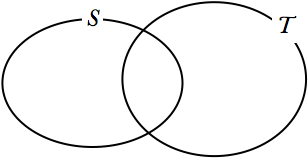
\includegraphics[scale=0.4]{FiguresMaths/setInitial}
        \caption{Two (overlapping) sets $S$ and $T$.}
        \label{fig:setInitial}
\end{center}
\end{figure}

\bigskip

\index{Venn diagram} \index{Venn, John}

\noindent \fbox{
\begin{minipage}{0.96\textwidth}
{\bf Explanatory note}.

Pictorial representations of sets such as those in Fig.~\ref{fig:setInitial} and its kindred illustrations are called {\it Venn diagrams}, in honor of John Venn, who employed them in his 1880 paper, ``On the diagrammatic and mechanical representation of propositions and reasonings", which appeared in the {\it Philosophical Magazine and Journal of Science}.
\end{minipage}
}

\bigskip

\noindent
We denote by:
\begin{itemize}
\item
$S \cap T$ the {\it intersection} of $S$ and $T$; see Fig.~\ref{fig:setIntersection}.
\begin{figure}[htb]
\begin{center}
        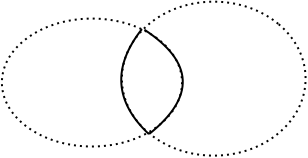
\includegraphics[scale=0.4]{FiguresMaths/setIntersection}
        \caption{Two operations on $S$ and $T$. The region within the bold border is their {\em intersection}. The region within the dotted border---excluding the bold lines---is their {\em symmetric difference}.}
        \label{fig:setIntersection}
\end{center}
\end{figure}

\smallskip

The elements of $S \cap T$ belong to {\em both} $S$ and $T$:
\[ [s \in S \cap T] \ \ \mbox{ means } \ \ 
\Big[ [s \in S] \ \mbox{\bf and } \ [s \in T] \Big]
\]

\item
$S \cup T$ the {\it union} of $S$ and $T$; see Fig.~\ref{fig:setUnion} .
\begin{figure}[htb]
\begin{center}
        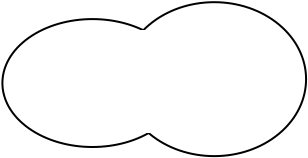
\includegraphics[scale=0.4]{FiguresMaths/setUnion}
        \caption{Union of sets $S$ and $T$.}
        \label{fig:setUnion}
\end{center}
\end{figure}

\smallskip

The elements of $S \cup T$ belong either to $S$, or to $T$, {\em or to both}:
\[ [s \in S \cup T] \ \ \mbox{ means } \ \
\Big[ [s \in S] \ \mbox{\bf or } \ [s \in T]  \ \mbox{\bf or } \ [s
    \in S \cap T] \Big]
\]
To emphasize the qualifier ``or to both'', this operation is sometimes called {\em inclusive union}. 
\index{set!operations!union} \index{set!operations!inclusive union}
\index{$S \cup T$: set union}
\item
$S \setminus T$ the {\em (set) difference} of $S$ and $T$; see Fig.~\ref{fig:setDiff}.
\begin{figure}[htb]
\begin{center}
        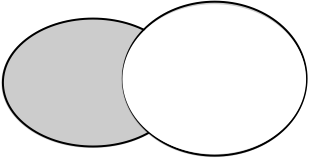
\includegraphics[scale=0.4]{FiguresMaths/setDiff}
        \caption{Difference of sets $S$ and $T$ (in grey).}
        \label{fig:setDiff}
\end{center}
\end{figure}

\smallskip

The elements of $S \setminus T$ belong to $S$ but {\em not} to $T$:
\[ [s \in S \setminus T] \ \ \mbox{ means } \ \
\Big[ [s \in S] \ \mbox{\bf and } \ [s \not\in T] \Big]
\]
(Particularly in the United States, one often encounters the notation ``$S-T$'' instead of ``$S \setminus T$''.)
 \index{$S \setminus T$: set difference} \index{$S - T$: set difference}
 \index{set!operations!set difference}
\end{itemize}

\medskip

\noindent 
We illustrate the preceding operations with the sets $S = \{a,b,c\}$ and $T = \{c,d\}$:\begin{eqnarray*}
S \cap T & = &  \{c\}, \\
S \cup T & = & \{a,b,c,d\}, \\
S \setminus T & = & \{a,b\}.
\end{eqnarray*}

\smallskip

In many situations where sets are being studied, the sets of interest will be subsets of some fixed ``universal'' set $U$.\index{set!universal set}

\bigskip

\index{Russell, Bertrand}
\noindent \fbox{
\begin{minipage}{0.96\textwidth}
{\bf Explanatory note}.

We use the term ``universal'' contextually, in the sense of a ``universe of discourse''.  We are {\em not} using the term in the absolute, self-referencing, sense of a set $U$ that contains all sets as members---``self-referencing'' because an absolute universal set $U$ would perforce contain itself as a member.  As we shall discuss in Section~\ref{sec:paradoxes}, the absolute, self-referencing, construct has been shown by the British philosopher/logician Bertrand Russell, to lead to the mind-bending paradox known eponymously as {\it Russell's Paradox} \cite{Russell02,Russell03}.
\end{minipage}
}
\bigskip

\index{$\overline{S}$: the complement of set $S$ relative to a universal set}
\noindent
Given a universal set $U$ and a {\em subset} $S \subseteq U$, we observe the set-inequalities
\[ \emptyset \ \subseteq \ S \ \subseteq \ U. \]
When we study a context within which there exists a universal set $U$, we include {\it (set) complementation} within our repertoire of set-related operations.
\index{set!operations!complementation}
\begin{itemize}
\item
$\overline{S} \ \eqdef \ U \setminus S$ is the {\em complement} of set $S$ (relative to the universal set $U$); see Fig.~\ref{fig:setComplement}.
\begin{figure}[htb]
\begin{center}
        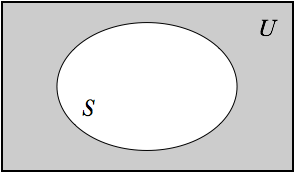
\includegraphics[scale=0.4]{FiguresMaths/setComplement}
        \caption{Complement of set $S$ (in grey) relative to the universal set $U$.}
        \label{fig:setComplement}
\end{center}
\end{figure}

\smallskip

$\overline{S} \ = \ U \setminus S$ is the set of all elements of $U$ that do not belong to $S$.  For instance, the set of {\em odd positive integers} is the complement of the set of {\em even positive integers}, relative to the set of {\em all positive integers}.
\end{itemize}

\bigskip

\noindent
We note a number of basic identities involving sets and operations on them.
\begin{itemize}
\item
$S \setminus T \ = \ S \cap \overline{T}$,
\item
If $S \subseteq T$, then
  \begin{enumerate}
  \item
$S \setminus T \ = \ \emptyset$,
  \item
$S \cap T \ = \ S$,
  \item
$S \cup T \ = \ T$.
  \end{enumerate}
\end{itemize}
Note, in particular, that\footnote{``iff'' is the common abbreviation for the mathematical phrase, ``if and only if.''}
\[ [S = T] \ \mbox{  iff  } \ \ \Bigl[[S \subseteq T] \mbox{
    {\small\sf and} } [T \subseteq S]\Bigr] \ \mbox{  iff  }
\ \ \Bigl[ (S \setminus T) \cup (T \setminus S) = \emptyset\Bigr].
\]

\medskip

\index{Boolean set operations} \index{Boole, George}
\index{set!operations!Boolean set operations} \index{set!operations!De Morgan's Laws}
\index{De Morgan's Laws} \index{De Morgan, Auguste}
The operations union, intersection, and complementation---and operations formed from them, such as set difference---are called the {\em Boolean (set) operations}, so named for the
$19$th-century English mathematician George Boole.  There are several important identities involving the Boolean set operations.  Among the most useful (hence, the most frequently invoked) are the two {\em laws} named for the $19$th-century French mathematician Auguste De Morgan:
\begin{equation}
\label{e.de-morgan}
\mbox{For all sets $S$ and $T$: } \ \left\{
\begin{array}{lcl}
\overline{S \cup T} & = & \overline{S} \cap \overline{T}, \\
 \\
\overline{S \cap T} & = & \overline{S} \cup \overline{T}.
\end{array}
\right.
\end{equation}
Elementary logic can be used to verify these laws.  To spell out just one case: An element $s$ that belongs to neither $S$ nor $T$ (so that $s \in \left(\overline{S} \cap \overline{T}\right)$) cannot belong to $S$ or to $T$, hence cannot belong to the union of $S$ and $T$.

\bigskip

\index{(Algebraic) Closure}
\noindent {\em (Algebraic) Closure}.
%
We end this section with a set-theoretic definition that one encounters in {\em many} contexts.
\begin{itemize}
\item
Let $\cal C$ be a (finite or infinite) collection of sets.
\item
Let $S$ and $T$ be elements of collection $\cal C$.\footnote{Note that $\cal C$ is a set whose elements are sets.}
\item
Let $\circ$ be an operation on sets---so that $S \circ T$ is a set.
\end{itemize}
We say that collection $\cal C$ is {\em closed} under the operation $\circ$ if whenever sets $S$ and $T$ (which could be the same set) both belong to $\cal C$, the set $S \circ T$ also belongs to $\cal C$.

\medskip

As a concrete example of the use of the notion of closure, we note the following.  De Morgan's laws tell us that a collection $\cal C$ of finite sets is closed under the operation of intersection whenever it is closed under the operations of union and complementation.

\section{Structured Sets}
\label{sec:structured-set}
\index{set!structured}

The power of set-theoretic concepts to model complex aspects of reality increases immeasurably when we consider sets whose elements enjoy even modest structure.  We begin our discussion of structured sets by adding a new (binary) set operation to our earlier repertoire.

\index{$S \times T$} \index{direct product of sets} \index{ordered pair of set elements}
 \index{Cartesian product of sets}

\smallskip

Given (finite or infinite) sets $S$ and $T$ we denote by $S \times T$ the {\it direct product} of $S$ and $T$, which is the set of all {\it ordered pairs} whose first coordinate is an element of set $S$ and whose second coordinate is an element of set $T$.  The direct product operation is often called the {\it Cartesian} product, because of the notion's origin in the formulation of Analytical Geometry by the French mathematician-philosopher Ren\'{e} Descartes. 
\index{Descartes, Ren\'{e}}

\smallskip

We illustrate the direct product operation in two ways, in order to capture all of its subtleties: Textually, if $S = \{a,b,c\}$ and $T = \{c,d\}$, then
\[ S \times T \ =  \{
\langle a,c \rangle,
\langle b,c \rangle,
\langle c,c \rangle,
\langle a,d \rangle,
\langle b,d \rangle,
\langle c,d \rangle\}
\]
Pictorially, Fig.~\ref{fig:cartesianproduct} provides a schematic illustration of $S \times T$.
\begin{figure}[htb]
\begin{center}
        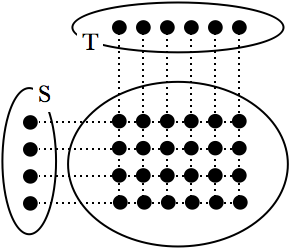
\includegraphics[scale=0.4]{FiguresMaths/cartesianProduct}
        \caption{The Direct/Cartesian product of sets $S$ and $T$.}
        \label{fig:cartesianproduct}
\end{center}
\end{figure}

\subsection{Binary Relations: Sets of Ordered Pairs}
\label{sec:relation}

\index{relation on sets} \index{binary relation on a set} \index{binary relation}
The direct-product operation on sets affords us a simple, yet powerful, formalization of the  notion of {\em binary relation}.  Given (finite or infinite) sets $S$ and $T$, a {\it relation $\rho$ on $S$ and $T$} (in that order) is any subset
\[ \rho \ \subseteq \ S \times T. \]
When $S = T$, we often call $\rho$ a {\em binary relation} \underline{on} {\em (the set) $S$}.  The qualifier ``{\em binary}'' indicates that relation $\rho$ establishes links between {\em pairs} of elements of set $S$.  (By extension, a {\em ternary} relation would establish links among {\em triples} of elements of $S$, and so on for larger -arities.) 

\smallskip

Relations are so common that we use them in every aspect of our lives without formally acknowledging the rules that govern them.  The relations ``equal to,'' ``less than,'' and ``greater than or equal to'' are simple examples of binary relations on the integers.  These same relations apply also to other familiar number systems such as the rational and real numbers; only the relation ``equals,'' though, holds (in the natural way) for the complex numbers.  (You will see much more about these sets of numbers in Chapters~\ref{ch:numbers-numerals}, \ref{ch:numbers-advanced}, and~\ref{ch:numerals}.)  Some subset of the three relations, ``is a parent of,'' ``is a child of,'' and ``is a sibling of'', are binary relations that may apply to (the set of people constituting) your family.  The preceding relations all apply to a single set $S$; a familiar relation for which the sets $S$ and $T$ are distinct is the relation ``$A$ is taking course $X$'', which is a relation on
\[ \left( \mbox{the set of all students} \right) \times \left( \mbox{the set of all courses} \right). \]

\ignore{************
We shall see later (Section~\ref{s.pairing}) that there is a formal
sense in which binary relations are all we ever need consider: $3$-set
({\em ternary}) 
relations\index{ternary relation}\index{relation!ternary}---which are
subsets of $S_1 \times S_2 \times S_3$---and $4$-set ({\em
  quaternary}) 
relations\index{quaternary relation}\index{relation!quaternary}---which
are subsets of $S_1 \times S_2 \times S_3 \times S_4$---and so on (for
any finite ``arity''), can all be expressed as binary relations of
binary relations \ldots of binary relations.  As examples: For ternary
relations, we can replace any subset $R$ of $S_1 \times S_2 \times
S_3$ by the obvious corresponding subset $R'$ of $S_1 \times (S_2
\times S_3)$: for each element $\langle s_1, s_2, s_3 \rangle$ of $R$,
the corresponding element of $R'$ is $\langle s_1, \langle s_2, s_3
\rangle \rangle$.  Similarly, for quaternary relations, we can replace
any subset $R''$ of $S_1 \times S_2 \times S_3 \times S_4$ by the
obvious corresponding subset $R'''$ of $S_1 \times (S_2 \times (S_3
\times S_4))$: for each element $\langle s_1, s_2, s_3, s_4 \rangle$
of $R''$, the corresponding element of $R'''$ is $\langle s_1, \langle
s_2, \langle s_3, s_4 \rangle \rangle \rangle$.
\begin{quote}
You should convince yourself that we could achieve the desired
correspondence also by replacing $S_1 \times (S_2 \times S_3)$ with
$(S_1 \times S_2) \times S_3$ and by replacing $S_1 \times S_2 \times
S_3 \times S_4$ by either $((S_1 \times S_2) \times S_3) \times S_4$
or $(S_1 \times S_2) \times (S_3 \times S_4)$.
\end{quote}
************}

\index{infix notation for a binary relation: $s \rho t$} 
\index{binary relation!infix notation}
By convention, when we deal with a binary relation $\rho \ \subseteq \ S \times T$, we often use {\em infix} notation: We write ``$s \rho t$'' in place of the more stilted ``$\langle s, t \rangle \in \rho$.''  For instance we (almost always) write ``$5 < 7$'' in place of the strange-looking (but formally correct) ``$\langle 5,7 \rangle \in \ <$.''

\medskip

\index{composition! binary relations} 
\index{composition of binary relations}
\index{binary relations!composition}

The following operation on relations occurs in many guises, in almost all areas of mathematics.  Let $\rho$ and $\rho'$ be binary relations on a set $S$.  The {\it composition} of relations $\rho$ and $\rho'$ (in that order) is the relation
\[ 
\rho'' \ \eqdef \ \Bigl\{ \langle s, t \rangle \in S \times S \ | \
(\exists u \in S) \Bigl[ [s \rho u] \mbox{ and } [u \rho' t] \Bigr] \Bigr\}.
\]
(Note that we use both of our notations for relations in this equation.) 

\bigskip

\noindent \fbox{
\begin{minipage}{0.95\textwidth}
{\bf Enrichment note}.

Even at this early stage in our study, we are using concepts that appear in ``real-life'' applications.  The operation of {\em composing relations} is an essential feature of {\it relational
  databases}, as described in the original source on the subject, \cite{Codd70}.  
\end{minipage}
}
\bigskip

\index{relation negation} \index{$\overline{\rho}$: the negation of relation $\rho$}
\noindent
When we discuss a relation $\rho \subset S \times T$, it is important to be able to express the assertion that elements $s \in S$ and $t \in T$ are {\em not} $\rho$-related.  We already have the elaborate notation, ``$\langle s, t \rangle \not\in S \times T$", but it would be good to have a streamlined notation also.  Several notations have been developed for this purpose, as the following table suggests.
\begin{equation}
\label{eq:NOT-rho-notation}
\begin{array}{|c|c|c|c|}
\hline
\mbox{\bf Relation} & \mbox{\bf Notation} & \mbox{\bf Negation}  \\
\hline
\hline
\mbox{set membership} & \in & \not\in  \\
\hline
\mbox{equality}       & =   & \neq     \\
\hline
\mbox{less than (strong)} & < & \not < \mbox{ or } \geq \\
\hline
\mbox{less than (weak)} & \leq & \not\leq \mbox{ or } >  \\
\hline
\mbox{greater than (strong)} & > & \not > \mbox{ or } \leq  \\
\hline
\mbox{greater than (weak)} & \geq & \not\geq \mbox{ or } <  \\
\hline
\mbox{generic}  & \rho  & \neg\rho \mbox{ or } \overline{\rho} \\
\hline
\end{array}
\end{equation}

\bigskip

Several special classes of binary relations are so important that we single them out immediately, in the upcoming subsections.


\subsection{Order Relations}
\label{sec:order-relation}

\index{order relation} \index{order relation!partial} \index{partial order} \index{order}
\index{transitive relation}

A binary relation $\rho$ on a set $S$ is a {\it partial order relation}, or, more briefly, is a {\it partial order} if $\rho$ is transitive.  This means that, for all elements $s, t, u \in S$,
\begin{equation}
\label{eq:def-transitive}
\mbox{\sf if } \ \ s \rho t \ \ \ \mbox{\sf \ and } \ \ \ t \rho u \ \ \ \mbox{\sf \ then }
\ \ \ s \rho u.
\end{equation}
The qualifier ``partial'' warns us that some pairs of elements of $S$ do not occur in relation $\rho$.  Number-related orders supply an easy illustration.  Given any two {\em distinct} integers, $m$ and $n$, one of them must be less than the other: i.e., either $m < n$, or $n < m$.  In contrast, if we consider {\it ordered pairs} of integers, then there are pairs of pairs that are not related by the ``less than'' relation in any natural way.  For instance, even though we may agree that---by a natural extension of the number-ordering relation ``less than''---the ordered-pair $\langle 4, 17 \rangle$ is ``less than'' the ordered-pair $\langle 22, 19 \rangle$, we may well not agree on which of the ordered-pairs $\langle 4, 22 \rangle$ and $\langle 19, 17 \rangle$ is ``less than'' the other.

\medskip

\index{order!strong}\index{order!weak}
\index{$\underline{\rho}$:the weak version of order relation $\rho$}
In many domains, order relations occur in two ``flavors'', {\em strong orders} and {\em weak orders}.  For many such relations $\rho$---consider, e.g., ``less than'' on the integers---the weak version is denoted by underscoring the strong version's symbol.  This will be our convention.  Just as $\leq$ denotes the weak version of $<$, and $\geq$ denotes the weak version of $>$, we shall denote the weak version of a generic order $\rho$ by the compound symbol $\underline{\rho}$.  Strong and weak versions of an order relation $\rho$ (denoted, respectively, $\rho$ and $\underline{\rho}$) are distinguished by their behavior under simultaneous membership.  For illustration, instantiate the following template with $\rho$ being ``$<$'' (less than) and with $\rho$ being ``$>$'' (more than):

\smallskip

\begin{tabular}{lll}
For a strong order $\rho$: & &
{\bf if} $[s \ \rho \ t]$, {\bf then} $[t \ \overline{\rho} \ s]$ \\
For the weak version $\underline{\rho}$ of $\rho$: & &
{\bf if} $[s \ \underline{\rho} \ t]$ {\bf and} $[t \ \underline{\rho}
  \ s]$, {\bf then} $[s = t]$.
\end{tabular}

\medskip

It is important to note that negating a strong relation (e.g., $<$) yields a weak relation ($\geq$), while negating a weak relation (e.g., $\leq$) yields a strong relation ($>$).  Keep this in mind when we study Propositional Logic in Section~\ref{sec:Propositional-logic}.  We shall note there that the following transformations
\begin{eqnarray*}
\mbox{weak order} + \mbox{negation} 
 & \longrightarrow & \mbox{strong order} \\
\mbox{strong order} + \mbox{negation}
 & \longrightarrow & \mbox{weak order}
\end{eqnarray*}
result from Proposition~\ref{thm:De-Morgan}, the logical analogue of De Morgan's Laws (\ref{e.de-morgan}).

\subsection{Equivalence Relations}
\label{sec:equiv-relation}

\index{equivalence relation} \index{relation!equivalence relation} 

A binary relation $\rho$ on a set $S$ is an {\it equivalence relation} if it enjoys the following three properties:

\medskip

\begin{tabular}{llll}
1. &
$\rho$ is {\em reflexive:}
   & $(\forall s \in S)$ & $[s \rho s]$ \\
2. &
$\rho$ is {\em symmetric:}
   & $(\forall s, s' \in S)$ 
& $\left[ [s \rho s'] \ \mbox{ iff } \ [s' \rho s] \right]$ \\
3. &
$\rho$ is {\em transitive:}
   & $(\forall s, s', s'' \in S)$ & if both \
$[s \rho s'] \ \mbox{ and } \ [s' \rho s''], \ \mbox{ then also } \ [s \rho s'']$
\end{tabular}

\medskip

\noindent
Sample familiar  equivalence relations are:
\begin{itemize}
\item
The equality relation $=$ on a set $S$.

\smallskip

This relation relates each $s \in S$ with itself (i.e., $s=s$) but with no other element of $S$.

\item
The relations $\equiv_{12}$ and $\equiv_{24}$ on integers, where\footnote{As usual, $|x|$ is the {\em absolute value}, or, {\em magnitude} of the number $x$: If $x \geq 0$, then $|x| = x$; if $x < 0$, then $|x| = -x$.}
  \begin{enumerate}
  \item
$n_1 \equiv_{12} n_2$ if and only if $|n_1 - n_2|$ is divisible by $12$.
  \item
$n_1 \equiv_{24} n_2$ if and only if $|n_1 - n_2|$ is divisible by $24$.
  \end{enumerate}

\smallskip

We use relation $\equiv_{12}$ (without formally acknowledging it) when we specify the time using a $12$-hour clock; we use relation $\equiv_{24}$ when we specify the time using a $24$-hour clock.
\end{itemize}

\smallskip

\index{partition} \index{set!partition}

\noindent
Closely related to the notion of an equivalence relation on a set $S$ is the notion of a {\it partition} of $S$---i.e., a nonempty collection of subsets $S_1, S_2, \ldots$ of $S$ that are

\smallskip

\begin{tabular}{l}
$\bullet$ {\em mutually exclusive:}
for distinct indices $i$ and $j$, $S_i \cap S_j = \emptyset$; \\
$\bullet$ {\em collectively exhaustive:}
$S_1 \cup S_2 \cup \cdots = S$.
\end{tabular}

\smallskip

\noindent
We call each set $S_i$ a {\it block} of the partition. \index{partition!block}
\index{set!partition!block} \index{block of a partition}

\noindent
One verifies the following Proposition easily.
\index{partitions!and equivalence relations} 
\index{equivalence relations!and partitions} 

\begin{prop}
A partition of a set $S$ and an equivalence relation on $S$ are just two ways of looking at the same concept.
\end{prop}

\begin{proof}[Sketch]
{\it To get an equivalence relation from a partition}.
Given any partition $S_1, S_2, \ldots$ of a set $S$, define the following relation $\rho$ on $S$:

\smallskip

$s \rho s'$ if and only if $s$ and $s'$ belong to the same block of the partition.

\smallskip

\noindent
We claim that relation $\rho$ is an equivalence relation on $S$.  To wit, the {\em collective exhaustiveness} of the partition ensures that each $s \in S$ belongs to some block of the partition, while {\em mutual exclusivity} ensures that $s$ belongs to only one block.

\medskip
\noindent {\it To get a partition from an equivalence relation}.
Focus on any equivalence relation $\rho$ on a set $S$.  For each $s \in S$, denote by $[s]_\rho$ the set
\[ [s]_\rho \ \eqdef \ \{ s' \in S \ | \ s \rho s' \} \]
we call $[s]_\rho$ the {\it equivalence class of $s$ under relation $\rho$}.
\index{equivalence class}\index{equivalence relation!class}

\smallskip

\noindent
{\em The equivalence classes under $\rho$ form a partition of $S$}.
To wit: $\rho$'s {\em reflexivity} ensures that the equivalence classes collectively exhaust $S$; $\rho$'s symmetry and transitivity ensure that equivalence classes are mutually disjoint.  \qed
\end{proof}

 \index{index (of an equivalence relation)}
\index{equivalence relation!index} \index{relation!equivalence relation!index} 
  
The {\it index} of the equivalence relation $\rho$ is its number of classes---which can be finite or infinite.  Henceforth, we conform to common usage and use the symbol $\equiv$, possibly embellished by a subscript or superscript, to denote an equivalence relation.

\smallskip

\index{refinement of an equivalence relation} 
\index{equivalence relation!refinement}

Let $\equiv_1$ and $\equiv_2$ be two equivalence relations on a set $S$.  We say that the relation $\equiv_1$ {\em is a refinement of}, or, {\em refines} the relation $\equiv_2$ precisely if each block of $\equiv_1$ is a subset of some block of $\equiv_2$.  We leave the verification of the following basic result as an exercise.

\begin{theorem}
\label{thm:equality=finest-equiv}
The equality relation, $=$, on a set $S$ is the {\em finest} equivalence relation on $S$, in the sense that $=$ refines every equivalence relation on $S$.
\end{theorem}

\subsection{Functions}
\label{sec:function}
\index{function}

\subsubsection{The basics: definitions and generic properties}
\label{sec:basic-functions}

One learns early in school that a function from a set $S$ to a set $T$ is a rule that assigns a unique value from $T$ to every value from $S$.  Simple examples illustrate that this notion of function is more restrictive than necessary.  Think, e.g., of the operation {\em division} on integers.  We learn that division, like multiplication, is a function that assigns a number to a given pair of numbers---yet we are warned immediately not to ``divide by $0$'': The quotient upon division by $0$ is ``undefined.''  So, division is {\em not quite} a function of the same sort as addition or multiplication, which both {\em do} conform to the notion envisioned by our initial definition of ``function''.  In more homely terms, note that, in contrast to an expression such as ``$4 \div 2$,'' which should lead to the result $2$ in every programming environment,\footnote{We are, of course, ignoring demons such as round-off error.}~expressions such as ``$4 \div 0$'' can lead to wildly different results in different programming environments.  Since ``wildly different'' is anathema in any mathematical setting, mathematicians have dealt with situations such as one encounters with division by broadening the definition of ``function'' in a way that behaves like our initial simple definition under ``well-behaved'' circumstances and that extends the notion in an intellectually consistent way under ``ill-behaved'' circumstances.  Let us begin to get formal.

\medskip

\index{function!source} \index{function!domain}
\index{function!target} \index{function!range}
A {\it (partial) function from set $S$ to set $T$} is a relation $F \subseteq S \times T$ that is {\it single-valued;} i.e., for each $s \in S$, there is {\em at most} one $t \in T$ such that $sFt$.  We
traditionally write ``$F: S \rightarrow T$'' as shorthand for the assertion, ``$F$ is a function from the set $S$ to the set $T$''; we also traditionally write ``$F(s) = t$'' for the more conservative (but
correct) ``$sFt$.''  (The single-valuedness of $F$ makes the nonconservative notation safe.)  We often call the set $S$ the {\em source}, or, {\it domain} of function $F$, and we call set $T$ {\em
  target} or, the {\it range} of function $F$.  In situations when there is always a (perforce, unique) $t \in T$ for each $s \in S$, then we call $F$ a {\em total} function.


\ignore{******* 
Note that our terminology is a bit unexpected: {\em Every total
  function is a partial function;} that is,
``partial''\index{function!partial} is the generic term, and ``total''
is a special case.
*********}

\medskip

You may be surprised to encounter functions that are not total, because most of the functions you deal with daily are {\em total}.  Our mathematical ancestors had to do some fancy footwork in order to make your world so neat.  Their choreography took two complementary forms.
\begin{enumerate}
\item
{\em They expanded the target set $T$ on numerous occasions.}

\smallskip

As just two instances:
  \begin{itemize}
  \item
They appended both $0$ and the negative integers to the preexisting positive integers in order to make subtraction a total function.

  \item
They appended the {\it rational numbers} to the preexisting integers in order to make division (by nonzero numbers!)~a total function.
  \end{itemize}
The {\it irrational algebraic numbers}, the {\it nonalgebraic real (or, transcendental) numbers}, and the {\it nonreal complex (or, imaginary) numbers} were similarly appended, in turn, to our number system in order to make certain (more complicated) functions total.  (Chapter~\ref{ch:numbers-numerals} expands on this brief history of our number system's development.)

\item
{\em They adapted the function.}

\smallskip

In programming languages, in particular, literal undefinedness is anathema---a computer must do {\em something}---so programming languages typically have chosen (sometimes artificial) ways of making functions total, via devices such as ``integer division'' (so that odd integers can be ``divided by $2$'') in additoin to various ploys for accommodating ``division by $0$.''
\end{enumerate}
The ($20$th-century) inventors of {\em Computation Theory} insisted on a theory of functions on nonnegative integers (or some transparent encoding thereof).  The price for such ``pureness'' is that they had to allow functions to be literally undefined on some arguments.  Thus the theory renders such functions as ``division by $2$'' and ``taking square roots'' as {\em nontotal}: Both are defined only on subsets of the positive integers (the even integers and the perfect squares, respectively).
\index{Computation Theory}

\medskip

Three special classes of functions merit explicit mention.  For each, we give both a down-to-earth name and a more scholarly Latinate one.
\begin{enumerate}
\item
A function $F: S \rightarrow T$ is {\it one-to-one}, or, {\it injective} if for each $t \in T$, there is at most one $s \in S$ such that $F(s) = t$;

\medskip

{\em Example:}
\begin{itemize}
\item
 ``multiplication by $2$'' is injective: If you are given an even integer $2n$, you can always respond with the integer $n$.
\item
``integer division by $2$'' is not injective---because performing the operation on arguments $2n$ and $2n+1$ yields the same answer (namely, $n$).
\end{itemize}

An injective function $F$ is called an {\it injection}.

\smallskip

\index{inverse of an injection}
\index{$F^{-1}$: functional inverse of injection $F$}

Importantly, each injection $F$ has a {\it functional inverse}, which is commonly denoted $F^{-1}$, and which is defined as follows.
\[
\mbox{For each $t \in T$:} \ \
F^{-1}(t) \ = \ \left\{
\begin{array}{cl}
s &
\mbox{ if there is an $s \in S$ such that $F(s) = t$} \\
\mbox{\it undefined } &
\mbox{ if there is no $s \in S$ such that $F(s) = t$}
\end{array}
\right.
\]
Because $F$ is {\em injective}, there is at most one element $s \in S$ such that $F(s)= t$.  In other words, an element $t \in T$ can occur in the range of $F$ only because of a single element $s \in S$ in the domain of $F$.  This means that
\begin{itemize}
\item
the preceding definition of $F^{-1}$ is a valid definition---i.e., the notion ``functional inverse of an injection'' is {\it ``well-defined''}.
\item
$F^{-1}$ is a (partial) function $F^{-1}: T \rightarrow S$ whose domain is the range of $F$.
\end{itemize}

\item
A function $F: S \rightarrow T$ is {\it onto} (or, {\it surjective}) if for each $t \in T$, there is at least one $s \in S$ such that $F(s) = t$;

\medskip

{\em Example:}
\begin{itemize}
\item
Two surjective functions on the nonnegative integers:
  \begin{itemize}
  \item
``subtraction of $1$'' is surjective, because ``addition of $1$'' is a total function.
  \item
``taking the square root'' is surjective because the operation of squaring is a total function.
  \end{itemize}
\item
Two functions on the nonnegative integers that are {\em not} surjective:
  \begin{itemize}
  \item
``addition of $1$'' is not surjective, because, e.g., $0$ is not ``$1$ greater'' than any nonnegative integer.
  \item
``squaring'' is not surjective, because, e.g., $2$ is not the square of any integer.  (We prove this as Proposition~\ref{thm:sqrt(2)}.) 
  \end{itemize}
\end{itemize}
A surjective function $F$ is called a {\it surjection}.

\item
A function $F: S \rightarrow T$ is ``{\it one-to-one, onto}" (or, {\it bijective}) if for each $t \in T$, there is precisely one $s \in S$ such that $F(s) = t$.

\ignore{**********
{\em Example:} The (total) function $F: \{0,1\}^\star \rightarrow
\{0,1\}^\star$ defined by:
\[
(\forall w \in \{0,1\}^\star) \ F(w) \ = \
\mbox{(the reversal of $w$)}
\]
is a bijection.  The (total) function $F': \{0,1\}^\star \rightarrow
\N$ defined by
\[
(\forall w \in \{0,1\}^\star) \ F(w) \ = \
\mbox{(the integer that is represented by $w$ viewed as a numeral)}
\]
is {\em not} a bijection, due to the possibility of leading $0$'s.
\begin{quote}
A {\it numeral}\index{representation of integers!numeral}
is a sequence of digits that is the ``name'' of a number.  The
numerical value of a numeral $x$ depends on the {\it number 
base},\index{representation of integers!number base}
which is a positive integer $b >1$ that is used to create $x$.  Much
of our focus will be on {\em binary} numerals---which are binary
strings---for which the base is 
$b=2$.\index{representation of integers!base-$2$ representation}\index{representation of integers!binary representation}
For a general number base $b$, the integer denoted by the numeral
$\beta_n \beta_{n-1} \ldots \beta_1 \beta_0$, where each $\beta_i \in
\{0,1, \ldots, b-1\}$, is\index{representation of integers!base-$b$ representation}
\[ \sum_{i=0}^n \ \beta_i b^i. \]
We say that bit $\beta_i$ has {\em lower order}\index{representation of integers!low-order bit}
in the numeral than does $\beta_{i+1}$, because $\beta_i$ is
multiplied by $b^i$ in evaluating the numeral, whereas $\beta_{i+1}$
is multiplied by $b^{i+1}$.
\end{quote}
*********}

A bijective function $F$ is called a {\it bijection}.  When $F$ is a bijection from $S$ onto $T$, we often write $F: S \leftrightarrow T$.
\end{enumerate}

\medskip

Finally, we present two terms that appear frequently in discussions of functions and their source and target sets.

\smallskip

\index{image, under a mapping} \index{preimage, under a mapping}
Focus on a function $f$ that maps a set $A$ {\em into} a set $B$; symbolically, we write $f: A \rightarrow B$.  The {\it image} of the set $A$ under $f$ is the subset of $B$
\[  \mbox{\sc image}(A) \ \eqdef \  \{f(a) \ | \ a \in A\} \]
The {\it preimage} of the set $B$ under $f$ is the subset of $A$
\[  \mbox{\sc preimage}(B) \ \eqdef \  \{a \in A \ | \ f(a) \in B\} \]


\smallskip

\index{permutation} \index{function!permutation}

\noindent
For any set $S$, a bijection $f: S \leftrightarrow S$ is called a {\it permutation} of set $S$.   Note that the set $S$ plays a lot of roles here: $S$ is:
\begin{itemize}
\item
the source of function $f$
\item
the target of function $f$
\item
the image of set $S$ under function $f$
\item
the preimage of set $S$ under function $f$
\end{itemize}


\subsubsection{$\oplus$ The Schr\"{o}der-Bernstein Theorem}
\label{sec:schroeder-bernstein}

This section is devoted to a remarkable theorem which states that {\em bijections} ($S \leftrightarrow T$) and {\em paired injections} ($S \rightarrow T$, $T \rightarrow S$) always travel together.  In detail, for all sets $S$ and $T$: If there exists both

\hspace*{.2in}{\em an injection from $S$ to $T$ and an injection from $T$ to $S$}

\noindent then there exists

\hspace*{.2in}{\em a bijection between $S$ and $T$}.

\index{The Schr\"{o}der-Bernstein Theorem}
\index{Bernstein, Felix}
\index{Schr\"{o}der, Ernst}
\index{The Cantor-Bernstein Theorem}
\index{Cantor, Georg}

\noindent
This is the celebrated theorem of Ernst Schr\"{o}der and Felix Bernstein; it is, alternatively, attributed to (Georg) Cantor and Bernstein.  As this complex attribution suggests, the theorem has a rather complicated history.  Picking just a few high points associated with the theorem's namesakes: The theorem was first stated without proof by Cantor in \cite{Cantor87}.  Roughly a decade later, Schr\"{o}der produced a flawed proof in \cite{Schroeder98a}.  As reported in \cite{Deiser2010}, Schr\"{o}der soon thereafter provided a correct proof---as, independently, did Bernstein.

We shall refer to the Theorem by its customary name, the {\it Schr\"{o}der-Bernstein Theorem}. This result can be immensely useful when reasoning about myriad mathematical scenarios that can be formulated using correspondences between the elements of two sets.  We encounter such a scenario, for example, when we prove Lemma~\ref{lem:N-=-F} in Section~\ref{sec:FNS-uncountable}.  Acknowledging the importance of the Theorem, we now provide a formal statement and a somewhat informal sketch of its proof.

\index{The Schr\"{o}der-Bernstein Theorem}
\begin{theorem}[The Schr\"{o}der-Bernstein Theorem]
\label{thm.S-B}
For any sets $S$ and $T$, if there exist both an {\em injection}
\[ F^{(S \rightarrow T)}: S \rightarrow T \]
and an {\em injection}
\[ F^{(T \rightarrow S)}: T \rightarrow S \]
then there exists a {\em bijection}
\[ F^{(S \leftrightarrow T)}: S \leftrightarrow T \]
\end{theorem}

\begin{proof}[Sketch]
We give the highlights of the perspicuous proof which appears in \cite{Tonien07}.

\smallskip

Let $S_0 = S$ and $T_0 = T$.  We set up a sequence of indices to orchestrate the upcoming argument: We have an index $i$ for each integer $i \in \N$, and we have a special index $\omega$ which takes care of the single case that the integer indices do not.

\ignore{\Denis we should add the range of $i$ here, start at 0 up to some integer denote by $\omega$}

For each index $i \in \N$, define
\[ S_{i+1} \ = \ F^{(T \rightarrow S)}(T_i) \ \ \ \ \mbox{ and }
\ \ \ \ T_{i+1} \ = \ F^{(S \rightarrow T)}(S_i) 
\]
We are repeatedly using here the notational convention that for any set $A$ and function $f$ defined on $A$,
\[ f(A) \ = \ \{ f(a) \ | \ a \in A \} \]
Because each of our injections, $F^{(S \rightarrow T)}$ and $F^{(T \rightarrow S)}$, maps its domain-set {\em into} its range-set (and not necessarily {\em onto}), we observe that increasing indices lead to nested progressions of sets, in the sense that
\[ \mbox{Each } \ \  S_{i+1} \subseteq S_i
 \ \ \ \mbox{ and each } \ \ \ 
 T_{i+1} \subseteq T_i
\]
We now define two new sequences of sets:
\begin{itemize}
\item
The sets $U_\omega$  and $U_0, \ U_1, \ U_2, \ldots$ are defined as follows:
\[ U_\omega \ = \ \bigcap_i S_i \ \ \ \ \
\mbox{and for each } \  i \in \N \ \ \  U_i \ = \ S_i \setminus S_{i+1} \]
Our reasoning shows that set $S$ is {\em partitioned} into the sets $U_0, \ U_1, \ U_2, \ldots$ and $U_\omega$.
\item
The sets $V_\omega$  and $V_0, \ V_1, \ V_2, \ldots$ are defined as follows:
\[ V_\omega \ = \ \bigcap_i T_i \ \ \ \ \
\mbox{and for each } \  i \in \N \ \ \  V_i \ = \ T_i \setminus T_{i+1}
\]
Our reasoning shows that set $T$ is {\em partitioned} into the sets $V_0, \ V_1, \ V_2, \ldots$ and $V_\omega$.
\end{itemize}
Moreover, one sees that:
\begin{itemize}
\item
$F^{(S \rightarrow T)}$ is a {\em bijection} between each $U_i$ and $V_{i+1}$, while
\item
$F^{(T \rightarrow S)}$ is a {\em bijection} between each $V_i$ and $U_{i+1}$.
\end{itemize}
Finally: Since $V_\omega \subseteq F^{(S \rightarrow T)}(S)$, and
\[ \Big[F^{(S \rightarrow T)}\Big]^{-1} (V_\omega) \ = \
\Big[F^{(S \rightarrow T)}\Big]^{-1} \Big(\bigcap T_{i+1} \Big) \ = \
\bigcap \Big[F^{(S \rightarrow T)}\Big]^{-1} (T_{i+1}) \ = \
\bigcap S_i \ = \ U_\omega
\]
it follows that $F^{(S \rightarrow T)}$ maps $U_\omega$ {\em bijectively} onto $V_\omega$.

\smallskip

Let us briefly ``decode" the preceding symbol-heavy chain of equations.  Recall first that $F^{(S \rightarrow T)}$ maps each set $S_i$ {\em injectively} into $T_{i+1}$.  This means that as we look at the {\it preimage} of the set $\bigcap T_{i+1}$ under $F^{(S \rightarrow T)}$, the various sets $S_i$ do not get ``mixed together"; they retain the separate identities that $F^{(S \rightarrow T)}$ endows them with because of the way it maps $S$ into $T$.  In other words,
\[ \Big[F^{(S \rightarrow T)}\Big]^{-1} \Big(\bigcap T_{i+1} \Big) \ = \
\bigcap \Big[F^{(S \rightarrow T)}\Big]^{-1} (T_{i+1}) \]

\ignore{\Denis right, but the interchanged of the inverse and the intersection is not obvious, may but a word here would be welcome?}

\smallskip

\noindent
By similar calculation and reasoning, $F^{(T \rightarrow S)}$ maps $V_\omega$ bijectively onto $U_\omega$.

\medskip

The preceding identifications of bijections between portions of set $S$ and portions of set $T$ allow us to piece together the advertised bijection $F^{(S \leftrightarrow T)}$ between the complete sets $S$ and $T$.  To wit:
\begin{itemize}
\item
For each $i \in \N$:
  \begin{itemize}
  \item
$F^{(S \leftrightarrow T)}$ maps each set $U_{2i}$ bijectively onto $V_{2i+1}$ in the same way that $F^{(S \rightarrow T)}$ does.
  \item
$F^{(S \leftrightarrow T)}$ maps each set $U_{2i+1}$ bijectively onto $V_{2i}$ in the same way that $F^{(T \rightarrow S)}$ does.
\end{itemize}

\item
$F^{(S \leftrightarrow T)}$ maps $V_\omega$ bijectively onto $U_\omega$ in the same way that either $F^{(S \rightarrow T)}$ or $\Big[F^{(T \rightarrow S)}\Big]^{-1}$ does.
\end{itemize}
This sketch provides all of the salient ingredients of the proof in \cite{Tonien07}.  \qed
\end{proof}
\ignore{\Denis nice and clear, just add the range of $i$ here (since it is bounded by $omega$}

\bigskip

\index{composition!functions} \index{function!composition}
While the operation of {\it (functional) composition}, as introduced in Section~\ref{sec:relation}, is important for general binary relations, it is a daily staple with relations that are functions!  Let us be given two functions on a set $S$
\[
F: S \rightarrow S \ \ \ \ \mbox{ and } \ \ \ \ G: S \rightarrow S
\]
The {\it composition} of $F$ and $G$, {\em in that order}, is the function
\[ F \circ G: S \rightarrow S \]
defined as follows.
\begin{equation}
\label{eq:functions-composed}
\mbox{For each } \ s \in S \ \ \
F \circ G(s) \ = \ G(F(s)).
\end{equation}
The unexpected change in the orders of writing $F$ and $G$ on the two sides of equation (\ref{eq:functions-composed}) results from the existence of two historical schools that both contributed to the formulation of this material.  One school cleaved to the tradition of {\it abstract algebra}:  they wanted expressions to be written with {\em all} operators, including the composition operator $\circ$, in {\em infix} notation---i.e., in the form ``$s \rho t$''.  Another school, which could be called the {\it applicative algebraic school}, wanted to view functions as ``applying'' to their arguments.  Both notations have significant advantages in certain contexts, so both have survived.  It is a good idea for neophyte readers to be prepared to encounter both notations---but they have to keep their eyes open regarding the relative orders of $F$ and
$G$.  \index{composition!functions!notation}

\medskip

Before we proceed with new material, let us take a moment to verify that the important operation of composition behaves the way one would want and expect it to---by preserving the type of function being composed.

\begin{prop}
\label{thm:fn-composition}
Let us be given functions $F: S \rightarrow S$ and $G: S \rightarrow S$ on the set $S$, together with their composition $F \circ G$, as defined in equation (\ref{eq:functions-composed}).

\noindent {\bf (a)}
$F \circ G$ is a function on $S$.

\noindent {\bf (b)}
If $F$ and $G$ are injections, then so also is $F \circ G$.

\noindent {\bf (c)}
If $F$ and $G$ are surjections, then so also is $F \circ G$.

\noindent {\bf (d)}
If $F$ and $G$ are bijections, then so also is $F \circ G$.
\end{prop}

\begin{proof}
We prove each of the four assertions by invoking the underlying definitions.

\noindent ({\bf a})
Because $F$ and $G$ are functions on $S$: For each $s \in S$, there is at most one $t_1 \in S$ such that $F(s) = t_1$ and at most one $t_2 \in S$ such that $G(s) = t_2$.  Hence, we identify three possibilities.

\smallskip

\begin{tabular}{lllll}
1. &
{\bf if}
$F$ is defined at $s \in S$  & & & {\bf then} $F(s) \in S$ is unique \\
  &
{\bf and if} $G$ is defined at $F(s) \in S$ & & & {\bf then} $G(F(s))
= F \circ G(s) \in S$ is unique \\
2. &
{\bf if}
$F$ is not defined at $s \in S$ & & & {\bf then} $F \circ G$ is not
defined at $s \in S$ \\ 
3. & 
{\bf if}
$F$ is defined at $s \in S$ & & & {\bf then} $F(s) \in S$ is unique \\
  &
{\bf and if} $G$ is not defined at $F(s) \in S$ & & & {\bf then}
$F \circ G$ not defined at $s \in S$ 
\end{tabular}

\smallskip

\noindent
Hence, for each $s \in S$, there is at most one $t \in S$ such that $F \circ G(s) = t$; in other words, $F \circ G$ is a function on $S$.

\medskip

\noindent ({\bf b})
Focus on any $s \in S$.  Because $F$ is an injection on $S$, there exists at most one $t \in S$ such that $F(t) = s$.  Because $G$ is an injection on $S$, there exists at most one $u \in S$ such that $G(u) = t$.  Thus, there exists at most one $u \in S$ such that $F \circ G(u) = s$.  Hence, $F \circ G(u)$ is an injection on $S$.

\medskip

\noindent ({\bf c})
Focus on any $s \in S$.  Because $F$ is a surjection on $S$, there exists $t \in S$ such that $F(t) = s$.  Because $G$ is a surjection on $S$, there exists $u \in S$ such that $G(u) = t$.  This means, however, that $F \circ G(u) = s$.  Because $s \in S$ was arbitrary, it follows that $F \circ G(u)$ is a surjection on $S$.

\medskip

\noindent ({\bf d})
If each of $F$ and $G$ is a bijection on $S$, then each is an injection on $S$, and each is a surjection on $S$.  Then Part (b) tells us that $F \circ G$ is an injection on $S$, and Part (c) tells
us that $F \circ G$ is a surjection on $S$.  Hence, $F \circ G$ is a bijection on $S$.  \qed
\end{proof}

\subsection{Sets, Strings, Functions: Important Connections}
\label{sec:sets-strings-functions}

\index{Shakespeare, William, {\it Romeo and Juliet}}
In his play, {\it Romeo and Juliet}, William Shakespeare pens a question whose significance goes far beyond its poetic origins: ``What's in a name?''  This section will hopefully get you thinking about that question in new ways!

Let us begin with a binary sequence---i.e., a sequence of bits
\[ \beta \ = \ \beta_0 \beta_1 \beta_2 \cdots \beta_n (\cdots) \]
where each $\beta_i \in \{0,1\}$.  The rather bizarre notation here, where the second set of (centered) dots is parenthesized, is intended to encompass both finite, length-$n$, sequences and infinite sequences.  The question is:

\smallskip

{\em What does sequence $\beta$ denote (or, name)?}

\smallskip

\noindent
At least three respectable answers to this question should be considered.
\begin{enumerate}
\item
With the most literal interpretation, $\beta$ is just an uninterpreted sequence of bits.

\item
With a little more imagination, one can interpret each bit $\beta_i$ of $\beta$ as information about the (index) integer $i$.  For example, $\beta$ can be viewed as specifying two mutually complementary sets of positive integers:
\begin{eqnarray*}
S_\beta \ = \ \{ k \in \N^+ \ | \ \beta_k = 1\} \\
\overline{S}_\beta \ = \ \{ k \in \N^+ \ | \ \beta_k = 0\}
\end{eqnarray*}
When $\beta$ has (finite) length $n$, then both $S_\beta$ and $\overline{S}_\beta$ are viewed as subsets of the set $\{1, 2, \ldots, n\}$; when $\beta$ is infinite, then both $S_\beta$ and $\overline{S}_\beta$ are viewed as subsets of the set $\N^+$.

\smallskip

In this scenario, $\beta$ is called the {\it characteristic sequence} of the set $S_\beta$.

\index{set!characteristic sequence}
\index{characteristic sequence (of a set)}

\medskip

\noindent {\em The notion of characteristic sequence leads to a quite simple way of counting the number of distinct subsets that an $n$-element set has.}

\smallskip

The number of length-$n$ binary strings is determined in Proposition~\ref{thm:b-ary strings} and is then used in Proposition~\ref{thm:power-sets} to count the subsets of an $n$-element set.

\item
Finally---{\em and we certainly do not mean to imply that our three alternatives exhaust the possibilities!}---each bit $\beta_i$ of $\beta$ can be interpreted as specifying the value at integer-argument $i$ of a function $f_\beta$.  When $\beta$ has (finite) length $n$, then $f_\beta$ is viewed as a function $f_\beta: \{1, 2, \ldots, n\} \rightarrow \{0,1\}$; when $\beta$ is infinite, then $f_\beta$ is viewed as a function $f_\beta: \N \rightarrow \{0,1\}$.

\smallskip

In this scenario, $\beta$ is called the {\it characteristic vector} of the function $f_\beta$.
\index{function!characteristic vector}
\index{characteristic vector!of a function}

\medskip

\noindent {\em The notion of characteristic vector leads to a rather straightforward proof that there does {\em not} exist a bijection between the set $\N^+$ of positive integers and the set of all functions from $\N^+$ to $\{0,1\}$, i.e., the set $\big\{ f:\N^+ \rightarrow \{0,1\} \big\}$.}  See Proposition~\ref{thm:R-uncountable}.
\end{enumerate}

We now have a new way to think about sequences/strings, sets, and functions.  Each way conveys insights and tools for reasoning about and analyzing these concepts that other ``names'' for the concepts do not.  And, we now recognize conceptual ties among these three concepts that are not always intuitive.  Our conceptual toolkit has been enriched!

\section{Boolean Algebras}
\label{sec:Boolean-Algebra}
\index{Boolean Algebra}

We remarked in Section~\ref{sec:operations-on-sets} that there is an extensive repertoire of operations on sets.  It is not difficult to compile a list of laws that various subsets of these operations obey.
\begin{itemize}
\item
The {\em commutativity} of union and intersection is one example:
\begin{eqnarray*}
S \cup T & = & T \cup S \\
S \cap T & = & T \cap S
\end{eqnarray*}

\item
The {\em distributivity} of either of union and intersection over the other provides another example:
\begin{eqnarray*}
R \cup (S \cap T) & = & (R \cup S) \cap (R \cup T) \\
R \cap (S \cup T) & = & (R \cap S) \cup (R \cap T)
\end{eqnarray*}

\smallskip

Notice that arithmetic (of numbers) has an analogue of the second of these equations---with multiplication playing the role of intersection and addition playing the role of union---but it does {\em not} have an analogue of the first.

\item
The {\em idempotence} of complementation provides a third example:
\[ \overline{\overline{S}} \ = \ S \]
\end{itemize}
Along the same general theme, there are special constants.
\[
\begin{array}{l}
S \cap \overline{S} \ = \ S \cap \emptyset \ = \ \emptyset \\
S \cup \overline{S} \ = \ S \cup U \ = \ U \ \mbox{ (the ``universal'' set)} \\
S \cup \emptyset \ = \ S \cup S \ = \ S \cap S \ = \ S \\
\end{array}
\]

\index{Boole, George}
The English logician/mathematician George Boole is historically credited with developing the system that we are describing here, with the goal of encapsulating a simple version of
mathematical logic within an algebraic framework; see
\cite{Boole54}.\footnote{The cited source seems to be an expansion on Boole's original exposition of these thoughts, in {\it The Mathematical Analysis of Logic} (1847).}  The system that Boole developed has been named {\it Boolean algebra}, in his honor.

Rather than provide an extensive description of ``abstract" Boolean algebras in terms of their operations and axioms, we turn directly to the system of logic that was Boole's inspiration and that has since his day provided a mathematical foundation for areas of immeasurable importance to technology.  (Much of an exposition of ``abstract" Boolean algebra would just repeat material from the ``applied" areas.)  We list citations to just three areas: the first citation is to Boole's original work; the other two are seminal studies by one of the greatest ``technology-theorists'' of the $20$th century, Claude E.~Shannon. \index{Shannon, Claude E.}
\begin{itemize}
\item
the foundations of mathematical logic \cite{Boole54}
\item
the mathematical foundations of switching-circuit theory \cite{Shannon38}
\item
the mathematical foundations of information theory \cite{Shannon48}
\end{itemize}
The genius of the mathematical system invented by Boole is manifest in the fact that it provides a starting point for formally understanding many seemingly disparate disciplines.  Indeed, if one develops a level of understanding of Boole's algebraic framework for Propositional Logic, then one can translate that understanding almost seamlessly to at least the preliminaries of Shannon's mathematical settings for Switching Circuit Theory and Information Theory.
\index{Switching Circuit Theory} \index{Information Theory}

\subsection{The Algebra of Propositional Logic}
\label{sec:Propositional-logic}
\index{propositional logic}\index{The Propositional Calculus}

\subsubsection{Logic as an algebra}
\label{sec:logic-as-algebra}

\paragraph{A. Propositions: the objects of the algebra}
\index{propositional logic!objects of the algebra}
\index{propositional logic!propositions}

\noindent
As we noted earlier in this chapter, what distinguishes Propositional
Logic from more general mathematical logic is the absence of
quantifiers ({\sc there exists}, {\sc for all}, etc.).  The objects of
Propositional Logic are {\it propositions}, i.e., fixed assertions, as
exemplified by the following three sentences.

\smallskip

\begin{tabular}{l}
``The sky is pink.'' \\
``Elephants are good swimmers.'' \\ 
``Colorless green dreams sleep furiously."
\end{tabular}

\index{Chomsky, Noam}

\bigskip

\noindent \fbox{
\begin{minipage}{0.96\textwidth}
{\bf Explanatory and Historical note}.

The property of being a ``proposition'' is {\em syntactic}, rather than {\em semantic}.  Our three sample propositions illustrate that the assertion made in a proposition need not be factually true---nor even sensible.  Indeed, the third of our samples was made famous by American linguist Noam Chomsky---in his seminal monograph {\it Syntactic Structures} (Mouton Press, 1957, {\it Janua Linguarum} series)---as he illustrated the independence of the notions ``grammatical" and ``meaningful".
\end{minipage}
}

\bigskip

The algebra that underlies Propositional Logic uses operations that are reminiscent of the set-theoretic operations to combine simple assertions into complex ones

\smallskip

{\bf if} ``the bananas are ripe'' {\bf and} ``you are hungry'' {\bf then} ``you should buy bananas''

\smallskip

{\bf either} ``the grass is green'' {\bf or} ``the ocean is calm''

\smallskip

\noindent
Two special propositions---the constants of the algebra---are denoted {\sc true} and {\sc false}.  They are {\em intended} to represent factual truth and factual falsehood, but they are {\em defined} by the way they interact with each other and with other propositions.  In order
to specify these interactions, we have to specify the logic's {\it connectives}: the operations of the algebra.

\bigskip

\paragraph{B. Logical connectives: the algebra's operations}
\index{propositional logic!operations of the algebra}
\index{propositional logic!logical connectives}

\noindent
As we describe and define the basic connectives of the Propositional Logic, we point out their relationships to the Boolean set-related operations introduced in Section~\ref{sec:operations-on-sets}.

\medskip

\index{logical operation!{\sc not} ($\neg$)}
\index{logical operation!negation}
\noindent {\sf B(i)} {\small\sf The {\em unary} logical connective}
\begin{itemize}
\item
\underline{{\sc not} ($\neg$)} or \underline{\it negation}
\hspace*{.1in}
{\small\sf (Set-theoretic analogue: {\em complementation})}.

\smallskip

Two shorthand notations for ``{\sc not} $P$'' have evolved:
  \begin{itemize}
  \item
the prefix-operator $\neg$, as in ``$\neg P$''
  \item
the overline-operator, as in ``$\overline{P}$''
  \end{itemize}
Whichever notation one uses, the defining properties of negation are encapsulated in the following equations.
\[
[\neg \mbox{\sc true} = \mbox{\sc false}] \ \ \mbox{ and } \ \ [\neg
  \mbox{\sc false} = \mbox{\sc true}].
\]
\end{itemize}

\medskip

\index{logical operation!{\sc or} ($\vee$)}
\index{logical operation!disjunction ($\vee$)}
\index{logical operation!logical sum ($\vee$)}
\noindent {\sf B(ii)} {\small\sf The {\em binary} logical connectives}
\begin{itemize}
\item
\underline{{\sc or} ($\vee$)} or \underline{\it disjunction}
\hspace*{.1in}
{\small\sf (Set-theoretic analogue: {\em union})}.

\smallskip

The operation {\sc or}---which is also called {\em logical sum}---is usually denoted by the infix-operator $\vee$; the operation's defining properties are encapsulated as follows.
\[
[[P \ \vee \ Q] =  \mbox{\sc true}] \ \ \mbox{ if, and only if, } \ \ 
[P = \mbox{\sc true}] \mbox{ or }
[Q = \mbox{\sc true}] \mbox{ or both}.
\]
Note that, as with union, logical {\sc or} is {\em inclusive:}  The assertion \\
\hspace*{.35in}$[P \vee Q]$ is \mbox{\sc true} \\
%
is true when {\em both} propositions $P$ and $Q$ are true, as well as when only one of them is.  Because such inclusivity does not always capture one's intended meaning, there is also an {\em exclusive} version of disjunction, as we see next.

\item 
\underline{{\sc xor} ($\oplus$)} or \underline{\it XOR}
\hspace*{.1in}
{\small\sf (Set-theoretic analogue: {\em disjoint union})}.
\index{logical operation!{\sc xor} ($\oplus$)}
\index{logical operation!exclusive or ($\oplus$)}

\smallskip

The operation {\em exclusive or} is a version of disjunction that does {\em not} allow both disjuncts to be true simultaneously.  It is usually denoted by the infix-operator $\oplus$; the operation's defining properties are encapsulated as follows.
\[
[[P \ \oplus \ Q] =  \mbox{\sc true}] \ \ \mbox{ if, and only if, } \ \ 
[P = \mbox{\sc true}] \mbox{ or }
[Q = \mbox{\sc true}] \mbox{ {\em but not} both}.
\]
We emphasize the distinction between $\vee$ and $\oplus$, the (respectively) inclusive and exclusive versions of disjunction, by remarking that the assertion
\[
[P \oplus Q]  \mbox{ is } \mbox{\sc true}
\]
is {\em false} when both propositions $P$ and $Q$ are true.

\item
\underline{{\sc and} ($\wedge$)} or \underline{\it conjunction}
\hspace*{.1in}
{\small\sf (Set-theoretic analogue: {\em intersection})}.
\index{logical operation!{\sc and} ($\wedge$)}
\index{logical operation!conjunction ($\wedge$)}
\index{logical operation!logical product ($\wedge$)}

\smallskip

The operation {\sc and}---which is also called {\em logical product}---is usually denoted by the infix-operator $\wedge$; the operation's defining properties are encapsulated as follows.
\[ [[P \ \wedge \ Q] = \mbox{\sc true}]  \ \ \mbox{ if, and only if,
  {\em both} } \ \ 
 [P = \mbox{\sc true}] \mbox{ and } [Q = \mbox{\sc true}]
\]

\item
\underline{{\sc implies}: logical implication ($\Rightarrow$)}
\hspace*{.1in}
{\small\sf (Set-theoretic analogue: {\em superset})}.
\index{logical operation!implies ($\Rightarrow$)}
\index{logical operation!implication ($\Rightarrow$)}
\index{logical operation!conditional ($\Rightarrow$)}
\index{logical operation!material implication ($\Rightarrow$)}

\smallskip

The logical operation {\sc implies}---which is often called {\it conditional}---is usually denoted by the infix-operator $\Rightarrow$; the operation's defining properties are encapsulated as follows.
\[ [[P \ \Rightarrow \ Q] = \mbox{\sc true}]  \ \ \mbox{ if, and only
  if, } \ \
  [ [\neg P] = \mbox{\sc true}] \mbox{ (inclusive) or } [Q = \mbox{\sc true}]
\]

We remark that the operation {\sc implies} differs from the other logical operations that we have discussed in a way that the reader must always keep in mind.  In contrast to {\sc not}, {\sc or}, {\sc xor}, and {\sc and}, whose formal meanings pretty much coincide with their informal meanings, the formal version of implication carries with it connotations that we do not always associate with the word ``implies'' in the vernacular.  One would not likely get universal agreement that the informal word ``implies'' satisfies the following properties that the formal word {\sc implies} definitely does.
  \begin{itemize}
  \item
{\em If proposition $P$  is false, then it implies {\em every} proposition.}
  \item
{\em If proposition $Q$ is true, then it is implied by {\em every} proposition.}
  \end{itemize}

\item
\underline{{\sc iff}: logical equivalence ($\equiv$)}
\hspace*{.1in}
{\small\sf (Set-theoretic analogue: {\em set equality})}.
\index{logical operation!is equivalent to ($\equiv$)}
\index{logical operation!biconditional ($\equiv$)}
\index{logical operation!if and only if ($\equiv$)}
\index{logical operation!iff ($\equiv$)}

The final logical operation that we shall discuss is known by many names, including {\it logical equivalence} and {\it biconditional}, as well as {\it if and only if} and its shorthand {\sc iff}.  It is usually denoted via one of the following two infix-operators: $\equiv$ or $\Leftrightarrow$; the operation's defining properties are encapsulated as follows.
\[ 
[[P \ \equiv \ Q] = \mbox{\sc true}]  \ \ \mbox{ if, and only if }
[[P \ \Rightarrow \ Q] = \mbox{\sc true}]  \ \ \mbox{ and } \ \
[[Q \ \Rightarrow \ P] = \mbox{\sc true}]
\]
Of course, our warnings concerning the tension between ``implies'' and {\sc implies} are inherited by {\sc iff} and its vernacular version.
\end{itemize}
\index{propositional logic!logic as a Boolean algebra}
\index{the Boolean algebra of logical operations}
\index{Boolean algebra!the Propositional Calculus}

\medskip

\index{The Propositional Calculus}
The Propositional Logic is often called the {\it Propositional Calculus}, acknowledging Boole's intention of developing an {\em algebra} of logic.  In the system Boole created, {\em logical connectives} become {\em algebraic operations}.  The ``set-theoretic analogues'' that we have specified in the course of introducing the logical connectives implicitly specify the laws that the Propositional operations obey.

\smallskip

As we shall discuss imminently, we never have to manipulate Propositional expressions algebraically in order to ``do" logic---although we are free to engage in such manipulation if we choose to.

\paragraph{C. The goal of the game: {\em Theorems}}
\index{propositional logic!theorem}
\index{logical system!theorem}

One learns as a student of either mathematics or mathematical logic that a {\it theorem} is a statement in the relevant logical system---in our case, the Propositional Calculus---such that one of the following is true:
\begin{itemize}
\item
The statement is an {\it axiom} of the system.\footnote{The word ``axiom'' means ``self-evident truth''.}
\item
The statement can be derived from the theorems of the system by repeated application of the system's rules of inference.
\end{itemize}
If this text were devoted to the topic of mathematical logic, then we would at this point develop the concepts that the preceding definition alludes to.  However, for us ``doers of mathematics", the Propositional Calculus is an avenue for introducing a variety of concepts within mathematics, not within mathematical logic.  Therefore, in the next section, we invoke (without proof) the powerful {\it Completeness Theorem for the Propositional Calculus} (Theorem~\ref{thm:Prop-calc-isfree}) which gives us access to a tremendous shortcut toward our goals.

\subsubsection{Semantic completeness: Logic via Truth Tables}
\label{sec:truth-tables}

\paragraph {A. Truth, theoremhood, and completeness}
\index{logical system!truth}
\index{logical system!interpretation}
\index{logical system!tautology}
\index{logical system!completeness}
\index{logical system!consistency}

Mathematical logic was invented to formalize the activity of mathematical reasoning.  The overarching goal was to develop a set of rules for ``playing the theorem-proving game'' in a way that was guaranteed to uncover true facts about whatever domain one was studying.  There are two complementary aspects to this goal:
\begin{enumerate}
\item
{\em to ensure that every theorem is true}

\smallskip

\index{logical system!consistency}

A logical system which achieves this goal is said to be {\it consistent}. 

\smallskip 

The main avenue to consistency is to ensure that the system's ``rules of inference'' combine simple expressions into complex ones in a way that preserves the truth of the expressions.  Of course, the algebra underlying the system plays a major role here.

\item
{\em to ensure that every true expression is a theorem}

\smallskip

\index{logical system!(semantic) completeness}

A logical system which achieves this goal is said to be {\it semantically complete}.  (There are other forms of logical completeness, but semantical completeness is a major---and natural---one.)

\smallskip

Regrettably, semantical completeness is a goal that is achievable only for the simplest logical systems.  Loosely speaking, no logical system that can correctly reason about elementary arithmetic propositions concerning integers, propositions such as

\smallskip

\hspace*{.25in}
``integer $n$ is the sum of integers $m$ and $p$''

\noindent or

\hspace*{.25in}
 ``integer $n$ is the product of integers $m$ and $p$''

\smallskip

\noindent {\em cannot be semantically complete}.  (Chapter~\ref{ch:arithmetic} contains a careful, but informal, discussion of incompleteness.)

\smallskip

In any semantically incomplete system of logic, there must be expressions that are {\em true but not provable}.
\end{enumerate}

\medskip

\noindent \fbox{
\begin{minipage}{0.96\textwidth}
{\bf Historical note}.

If the preceding discussion surprises you, then you are in good company.  The publication that announced the incompleteness result, \cite{Goedel31}, turned the mathematical world on its ear when it appeared in 1931!
\end{minipage}
}

\bigskip

Happily for many mathematical and computational goals, the Propositional Calculus is sufficiently simple that it {\em is} semantically complete.  We elaborate a bit on this fact now.

\paragraph{B. The completeness of Propositional Logic}
\index{logical system!completeness}

The {\em semantic completeness} of the Propositional Calculus as a logical system is a consequence of the fact that we are able to view the expressions of the Calculus as Boolean functions, in the following way.
\begin{itemize}
\item
All propositions, $P$, $Q$, \ldots, that appear in expressions are uninterpreted ``names'' of actual propositions.
\item
As we examine an expression in the Calculus, the only information we need about the propositions $P$, $Q$, \ldots, which appear in the expression is the array of truth-values for the propositions.
\end{itemize}
If we tabulate how the truth-values of propositions combine under the logical operators that interconnect them in the expression, then we remark immediately how the expressions can be viewed as {\em functions of binary tuples}, where the -arity of the functions is the number of propositional variables.  Using this viewpoint, the tables in Fig.~\ref{fig:defns-via-tables} reproduce the definitions of the logical operators of Section~\ref{sec:logic-as-algebra}.B, viewed as functions within the space of truth-values.  Each propositional variable is instantiated with all of its possible truth-values, {\sc true} and {\sc false}---which we denote here, for convenience, as $1$ and $0$, respectively.
\begin{figure}[hbt]
\[
\begin{array}{|c||c|}
\hline
P & \neg P \\
\hline
\hline
0 & 1 \\
\hline
1 & 0 \\
\hline
\end{array}
\hspace*{.5in}
\begin{array}{|c|c||c||c||c||c||c|}
\hline
P & Q & P \vee Q  & P \oplus Q & P \wedge Q & P \Rightarrow Q & P \equiv Q  \\
\hline
\hline
0 & 0 & 0 & 0 & 0 & 1 & 1 \\
\hline
0 & 1 & 1 & 1 & 0 & 1 & 0 \\
\hline
1 & 0 & 1 & 1 & 0 & 0 & 0 \\
\hline
1 & 1 & 1 & 0 & 1 & 1 & 1 \\
\hline
\end{array}
\]
\caption{Tabular presentations of the basic Propositional connectives.
\label{fig:defns-via-tables}}
\end{figure}
Note how the truth-value entries in the righthand truth table of Fig.~\ref{fig:defns-via-tables} reinforce the lessons of Section~\ref{sec:logic-as-algebra}.B.  This awareness is essential with the implication-related operations ($\Rightarrow$ and $\equiv$) in the light of our earlier discussion of the tension between their formal meanings (from the table) and the way they are
used in ``real-life'' reasoning voiced in the vernacular.

\medskip

\index{tautology} \index{propositional logic!tautology}
\index{Satisfiable logical expression} 
\index{satisfiable propositional expression} 
\index{propositional logic!satisfiable expression}
Every Propositional expression is a binary function, so we can pass back and forth between logical and functional/operational terminology.  This ability affords us very simple definitions of two important concepts that are somewhat harder to define in purely logical terms.
\begin{itemize}
\item
{\sf Tautology}. 
  \begin{itemize}
  \item
{\it Mathematical formulation:}

\smallskip

A Propositional expression is a {\it tautology} iff its corresponding function is the constant function $F(x) \equiv 1$.
  \item
{\it Logical formulation:}

\smallskip

A Propositional expression is a {\it tautology} iff it evaluates to {\sc true} under every instantiation of truth-values for its Propositional variables.
  \end{itemize}
\item
{\sf Satisfiable expression}.
  \begin{itemize}
  \item
{\it Mathematical formulation:}

\smallskip

A Propositional expression is {\it satisfiable} iff its corresponding function has $1$ in its range; i.e., iff there is an argument $x$ such that $F(x) = 1$.
  \item
{\it Logical formulation:}

\smallskip

A Propositional expression is {\it satisfiable} iff there exists an instantiation of truth-values for its Propositional variables under which the expression evaluates to {\sc true}.
  \end{itemize}
\end{itemize}

\medskip

\noindent
We are now ready to present the main result of this section.

\begin{theorem}[The Completeness Theorem for Propositional Logic]
\label{thm:Prop-calc-isfree}
A Propositional expression $E(P, Q, \ldots, R)$ is a theorem of Propositional logic if, and only if, it is a tautology.
\end{theorem}

Proving Theorem~\ref{thm:Prop-calc-isfree} is beyond the scope of this book.  The interested reader can find a proof in myriad logic texts.  The proof in  \cite{Rosser53} might be particularly interesting to an aspiring mathematician because that source exists precisely to explain logic in terms that are accessible to a mathematician.

\bigskip

The next subsection presents illustrative applications of the Theorem.

\paragraph{C. The laws of Propositional logical as theorems}
\index{logical operations!a functional view}

The applications of Theorem~\ref{thm:Prop-calc-isfree} which we have chosen to discuss here are the {\em laws} of the logical algebra described in Section~\ref{sec:Propositional-logic}.

\bigskip

\index{propositional logic!truth tables!law of double negation}
\index{truth tables!law of double negation}
\noindent
\underline{\small\sf The law of double negation}

\smallskip

\noindent
This is a formal analogue of the homely adage that ``a double negative is a positive.''

\begin{prop}
\label{thm:double negation}
For any proposition $P$,
\[ P \ \ \equiv \ \ \neg [\neg P] \]
\end{prop}

\noindent {\it Proof via truth table.}
\begin{equation}
\label{eq:double-neg}
\begin{array}{|c|c||c|}
\hline
P & \neg P & \neg[\neg P] \\
\hline
\hline
0 & 1 & 0 \\
\hline
1 & 0 & 1 \\
\hline
\end{array}
\end{equation}
Note that columns 1 and 3 of truth table (\ref{eq:double-neg}) are identical.  By Theorem~\ref{thm:Prop-calc-isfree}, this fact verifies Proposition~\ref{thm:double negation}, the law of double negation.  \qed

\bigskip

\index{propositional logic!truth tables!law of contraposition}
\index{truth tables!law of contraposition}
\noindent 
\underline{\small\sf The law of contraposition}

\smallskip

\noindent
This is a very exciting example!  Let us immediately convert this to a mathematical statement about the Boolean Algebra of Propositional logic and then prove the statement.  We shall then contemplate the implications of this law for {\em logic} rather than {\em mathematics}.
\index{contraposition!in the Boolean Algebra of propositions}

\begin{prop}
\label{thm:contraposition}
For any propositions $P$ and $Q$,
\[  \left[ [ P \Rightarrow Q ] \ \ \equiv \ \ [ \neg Q
    \Rightarrow \neg P ] \right]
\]
\end{prop}

\noindent {\it Proof via truth table.}
\begin{equation}
\label{eq:contraposition}
\begin{array}{|c|c|c|c||c||c|}
\hline
P & \neg P & Q & \neg Q & \underline{P \Rightarrow Q}
 & \underline{\neg Q \Rightarrow \neg P} \\
\hline
\hline
0 & 1 & 0 & 1 & 1 & 1 \\
\hline
0 & 1 & 1 & 0 & 1 & 1 \\
\hline
1 & 0 & 0 & 1 & 0 & 0 \\
\hline
1 & 0 & 1 & 0 & 1 & 1 \\
\hline
\end{array}
\end{equation}
Note that columns 5 and 6 of truth table (\ref{eq:contraposition}) are identical.  By Theorem~\ref{thm:Prop-calc-isfree}, this fact verifies Proposition~\ref{thm:contraposition}, the law of contraposition.  \qed

\smallskip

Now let us reconsider the whole concept of contraposition, including this law, in the light of {\em logic and reasoning}.
\index{contraposition!in logic, reasoning}
\index{Law of contraposition}

\medskip

The {\it Law of Contraposition} states that the assertion

\smallskip

\hspace*{.35in}
``Proposition $Q$ implies Proposition $Q$''

\smallskip

\noindent
is {\em logically equivalent} to the assertion

\smallskip

\hspace*{.35in}
``the negation of Proposition $Q$ implies the negation of Proposition $P$''.

\smallskip

\noindent
Think about this!  This is a version of Proof by Contradiction!

\bigskip

\noindent 
\underline{\small\sf De Morgan's Laws}:
\index{propositional logic!Truth tables!verify De Morgan's laws}
\index{truth tables!verify De Morgan's laws}

\begin{prop}
\label{thm:De-Morgan}
For any propositions $P$ and $Q$:
\begin{itemize}
\item
$[ P \wedge Q ] \ \ \equiv \ \ \neg [ [\neg P] \vee [\neg Q]]$
\item
$[ P \vee Q ] \ \ \equiv \ \ \neg [ [\neg P] \wedge [\neg Q]]$
\end{itemize}
\end{prop}

\noindent {\it Proof via truth table.}
\begin{equation}
\label{eq:DeMorgan}
\begin{array}{|c|c|c|c||c|c|||c|c|}
\hline
P & \neg P & Q & \neg Q 
  & [ P \wedge Q ]
  & [\neg P] \vee [\neg Q]
  & [ P \vee Q ]
  & [\neg P] \wedge [\neg Q] \\
\hline
\hline
0 & 1 & 0 & 1
  & 0
  & 1
  & 0
  & 1 \\
\hline
0 & 1 & 1 & 0
  & 0
  & 1
  & 1
  & 0 \\
\hline
1 & 0 & 0 & 1
  & 0
  & 1
  & 1
  & 0 \\
\hline
1 & 0 & 1 & 0
  & 1
  & 0
  & 1
  & 0 \\
\hline
\end{array}
\end{equation}
Note that columns 5 and 6 of truth table (\ref{eq:DeMorgan}) are mutually complementary, as are columns 7 and 8.  If we negate (or, complement) the entries of columns 6 and 8, then we can invoke Theorem~\ref{thm:Prop-calc-isfree} to verify proposition~\ref{thm:De-Morgan}, which encapsulates De Morgan's laws for Propositional logic.  \qed

\medskip

\noindent 
\underline{\small\sf The distributive laws for Propositional logic}
\index{propositional logic!truth tables!distributive laws}
\index{truth tables!distributive laws for propositional logic}

\smallskip

\noindent
In numerical arithmetic, multiplication distributes over addition, but not conversely, so we have a single distributive law for arithmetic (see Section~\ref{sec:Arithmetic-Laws}).  In contrast, each of logical multiplication and logical addition distributes over the other, so we have {\em two} distributive laws for Propositional logic.
\begin{itemize}
\item
$ P \vee [ Q \wedge R] \ \ \equiv \ \ [P \vee Q] \wedge R$
\item
$P \wedge [ Q \vee R] \ \ \equiv \ \ [P \wedge Q] \vee R$
\end{itemize}
{\small
\begin{equation}
\label{eq:distrib-law}
\begin{array}{|c|c|c||c|c|c|c|||c|c||c|c|}
\hline
P & Q & R
  & [P \vee Q]
  & [P \wedge Q]
  & [Q \wedge R] 
  & [Q \vee R] 
  & P \vee [ Q \wedge R]
  & [P \vee Q] \wedge [P \vee R]
  & P \wedge [ Q \vee R]
  & [P \wedge Q] \vee [P \wedge R] \\
\hline
\hline
0 & 0 & 0
  & 0
  & 0
  & 0
  & 0
  & 0
  & 0
  & 0
  & 0 \\ 
\hline
0 & 0 & 1
  & 0
  & 0
  & 0
  & 1
  & 0
  & 0
  & 0 
  & 0 \\
\hline
0 & 1 & 0
  & 1
  & 0
  & 0
  & 1
  & 0
  & 0
  & 0
  & 0 \\
\hline
0 & 1 & 1
  & 1
  & 0
  & 1
  & 1
  & 1
  & 1
  & 0
  & 0 \\
\hline
1 & 0 & 0
  & 1
  & 0
  & 0
  & 0
  & 1
  & 1
  & 0
  & 0 \\
\hline
1 & 0 & 1
  & 1
  & 0
  & 1
  & 0
  & 1
  & 1
  & 1
  & 1 \\
\hline
1 & 1 & 0
  & 1
  & 1
  & 0
  & 1
  & 1
  & 1
  & 1
  & 1 \\
\hline
1 & 1 & 1
  & 1
  & 1
  & 1
  & 1
  & 1
  & 1
  & 1
  & 1 \\
\hline
\end{array}
\end{equation}
}

Note that columns 8 and 9 of truth table (\ref{eq:distrib-law}) are identical, as are columns 10 and 11.  By Theorem~\ref{thm:Prop-calc-isfree}, this fact verifies the distributive laws for Propositional logic.


\subsection{$\oplus \oplus$ A Purely Algebraic Setting for Completeness}

In the hope of whetting the appetite of at least some readers, we remark here that there is a rather sophisticated algebraic concept that can be used to derive Theorem~\ref{thm:Prop-calc-isfree} in a purely algebraic setting.  We have noted that the Propositional Calculus is a Boolean Algebra.  One can state more: the Propositional Calculus is a {\em free} Boolean Algebra.
\index{Boolean Algebra!free algebra}

\smallskip

The meaning of the qualifier {\it free} is easy to state but not so easy to understand.  Here is a very informal try.

\smallskip

An algebra of type $X$---in our case, $X$ is a Boolean Algebra---is {\em free} if it obeys no laws except those that it must obey to belong to the class of type-$X$ algebras.

\smallskip

\index{axioms as ``self-evident truths''}

In more detail: \\
Any genre of algebra is defined as a set of objects accompanied by a set of basic operations, which obey certain ``self-evident'' axioms.  In rough, but evocative, terms, the algebra is {\em free} if its operations do not relate to one another in any way that is not mandated by the axioms.

\smallskip

\index{semi-group} \index{associative law}

Here is an easy illustration of this decidedly {\em not-easy} concept.  There is a (quite important) genre of algebra called a {\it semi-group}.  A semi-group $\s$ is specified via a set (of objects) $S$, together with a binary operation on $S$, which we denote $\otimes$.  For the (algebraic) structure $\s = \langle S, \otimes \rangle$ to be a semi-group, it must obey the following two laws.
\begin{enumerate}
\item
$\s$ must be {\it closed} under operation $\otimes$; i.e., for all $s_1, s_2 \in S$, we must have
\[ (s_1 \otimes s_2) \in S. \]
\item
The operation $\otimes$ must obey the {\em associative law;} i.e., for all $s_1, s_2, s_3 \in S$,
\[ (s_1 \otimes s_2) \otimes s_3 \ = \ s_1 \otimes (s_2 \otimes s_3) \]
\end{enumerate}

Now, it is easy to verify---we shall discuss this in Chapter~\ref{ch:arithmetic}---that the (algebraic) structure formed by the integers coupled with the operation of addition forms a semi-group (which the notation of Chapter~\ref{ch:arithmetic} would denote $\langle \Z, + \rangle$).  But this semi-group is {\em not} free, because integer addition obeys laws beyond just closure and associativity, namely:
\begin{enumerate}
\item
Addition of integers is {\em commutative}.
\item
Integer addition has an {\em identity}, namely $0$.
\item
Every integer $z \in \Z$ has an {\it additive inverse} (namely, $-z$).
\end{enumerate}

So, it {\em is} meaningful---and consequential---that the Propositional calculus is a {\em free} Boolean algebra.


\subsection{Satisfiability Problems and {\sf NP}-Completeness}
\label{sec:Satisfiability}

\index{logical expressions!truth values}
\index{logical expressions!logical variables}
\index{logical expressions!logical literals}
\index{logical expressions!logical literals!true or complemented}

Satisfiability problems deal with propositional formulae that are populated by entities that can assume the truth values {\sc true} and {\sc false}.  The {\em underlying} entities are {\it logical variables}, i.e., variables that range over the truth values.  The {\em actual} entities that appear in each formula are {\it logical literals}, i.e., \underline{\em instances of logical variables} in either their {\em true} or {\em complemented} forms.  In detail:
\begin{itemize}
\item
In its {\em true} form, a literal evaluates to {\sc true} precisely when its associated variable does.
\item
In its {\em complemented} form, a literal evaluates to {\sc true} precisely when its associated variable evaluates to {\sc false}.
\end{itemize}
The following simple examples should clarify these terms.

\begin{tabular}{ll}
{\small\sf The formula}:  & $(\neg {x} \vee y) \wedge (x \vee \neg{y})$ \\
{\small\sf The variables}: & $x$ and $y$ \\
{\small\sf The literals}:  & $x$ and $y$ (true form); \ $\neg {x}$ and $\neg {y}$
(complemented form)
\end{tabular}
\[
\begin{array}{ccccccccccc}
( & \neg {x} & \vee & y & ) & \wedge & ( & x & \vee & \neg{y} & ) \\
  & \uparrow &     & \uparrow & & & & \uparrow & & \uparrow & \\
  & \mbox{complemented} &  & \mbox{true}  & & & & \mbox{true} &
        & \mbox{complemented} &  \\
  & \mbox{literal} & & \mbox{literal} & & & & \mbox{literal} & &
  \mbox{literal} & 
\end{array}
\]

\smallskip

\noindent {{\sf SAT}: {\small\sf The original {\sf NP}-complete problem}

\index{The Satisfiability Problem (for the Propositional Calculus)}
\index{{\sf SAT}} \index{{\sf SAT}!definition} \index{{\sf SAT}: The Satisfiability Problem} \index{Satisfiability problem!combinatorial formulation}
\index{{\sf SAT}!combinatorial formulation}
\index{Satisfiability problem!formal logical formulation}
\index{{\sf SAT}!formal logical formulation}

\noindent
The general form of {\it The Satisfiability Problem for the Propositional Calculus} is denoted {\sf SAT}.  The problem can be viewed in two formally distinct but algorithmically equivalent ways.
\begin{itemize}
\item
In the {\it combinatorial formulation}:
  \begin{itemize}
  \item
The Satisfiability Problem is specified by a set of {\it logical clauses}, each clause being a {\it set of {\em logical} variables}, i.e., variables that range over the truth values {\sc true} and {\sc false}.
  \item
The Satisfiability question is: Can one assign truth values to all of the logical variables of the formula in such a way that every clause ends up with at least one {\sc true} literal?
  \end{itemize}
\item
In the {\it formal logical formulation}:
  \begin{itemize}
  \item
The Satisfiability Problem is specified by a propositional formula $\Phi$ that is  a {\it conjunction of disjuncts of logical literals}.

\smallskip

\index{POS-form expression} 
 
In the lingo of the {\em cognoscenti} (the ``in-crowd''), these expressions are said to be in {\it POS} form, shorthand for a {\it (logical) product of (logical) sums}.
  \item
The Satisfiability question is: Can one assign truth values to all of the logical variables of formula $\Phi$ in such a way that every disjunct evaluates to {\sc true}?
  \end{itemize}
\end{itemize}
The reader should be able to prove that these are just two views of the same logical problem.

\bigskip

\index{SOP-form expression}
\index{Cook, Stephen A.}

Until 1971, POS expressions were largely viewed simply as the duals of the somewhat more common {\it SOP}-form expressions, shorthand for {\it sums of products}.   A discovery in 1971 by Stephen A.~Cook changed this view: Cook exposed, in \cite{Cook71}, how POS-form expressions can be used to model a number of computational phenomena whose importance
was only beginning to be understood at that time.  These phenomena were {\it nondeterminism in computation} and {\it computational complexity}.
\index{nondeterminism in computation} 
\index{computational complexity}

\medskip

{\it Nondeterminism} can best be thought of in one of the following ways.  The first, more concrete, way to think about a nondeterministic computing device is as a device that can ``make guesses'' at various junctures of a computation, rather than performing some prolonged search through plausible alternative fixed paths.  The second, more idealistic, way to think about a nondeterminism is by imagining that a computing device has the capability of spawning alternative universes that it can proceed through ``in parallel.''

\bigskip

\noindent \fbox{
\begin{minipage}{0.96\textwidth}
{\bf Explanatory note}.

We place the phrase ``in parallel'' within quotes because parallel computing is a concrete computational paradigm, while nondeterministic computing is a purely conceptual framework for thinking about the computational process.
\end{minipage}
}
\bigskip

\index{finite automata} \index{Rabin, Michael O.}  \index{Scott, Dana}
 
\noindent 
Nondeterminism was invented during the 1950s, under a variety of names, as a conceptual framework for understand the computing power of {\it finite automata}.  The concept's
appearance in the seminal study \cite{RabinS59} by Michael O.~Rabin and Dana Scott
established the standard way of formulating and discussing the topic.

\medskip

By the early 1960s, computation theorists had recognized the importance of developing conceptual, mathematical, tools for discussing, analyzing, and quantifying the {\em complexity} of performing computations.  For close to a decade, models for studying such issues were proposed, discarded, improved, and embellished, but no consensus developed about an intellectually uniform approach to the topic.  This situation largely changed toward the end of the 1960s.  The issues were split into what one might term {\em concrete} questions, which focused on specific computational problems and specific computing platforms, and what one might term {\em abstract} questions, which tried to uncover foundational insights into what made---or appeared to make---certain types of computational problems {\em inherently} difficult.  Substantial progress was made on the concrete front, but the abstract front proved quite recalcitrant until Cook's work at the end of the decade.

\medskip

\index{computational complexity} 
\index{computability theory}
\index{computation theory}
\index{G\"{o}del, Kurt} \index{Turing, Alan M.}
In 1971, Cook announced, in \cite{Cook71}, a revolutionary foundation for the field of {\it computational complexity}, which built upon the conceptual frameworks\footnote{These frameworks were the legacy of intellectual giants such as Kurt G\"{o}del (in \cite{Goedel31}) and Alan M.~Turing (in \cite{Turing36}).}~of the decades-old field known variously as {\it computability theory}  and {\it computation theory}.   Computability theory enabled one to study questions about the {\em feasibility} of computing a function $f$,

\smallskip

\noindent
Can one write a program that will enable a digital computer to compute function $f$?

\smallskip

 \index{{\sf NP}-completeness}
\index{{\sf NP}-complete computational problems}

\noindent
Cook's new theory enabled one to rigorously study a range of questions regarding the {\em efficiency} that could be achieved by a digital computer as it performs a (perforce, feasible) computation.  One could now ask the following types of questions about the {\em complexity} of computations for functions $f$ and $g$:
\begin{itemize}
\item
Why is it easy (computationally) to prove that $f(x) = y$, but hard to compute $f(x)$?
\item
Why can you adapt any program that computes function $f$ to a ``similar'' program that computes function $g$, even though these functions do not apparently have any relationship to one another?
\item
Is function $f$ inherently harder to compute than function $g$?
\end{itemize}
Cook's ingenious adaptation created a new theory that was named (the theory of) {\it {\sf NP}-completeness}, for reasons that are explained in sources such as \cite{GareyJ79}.  In very informal, but hopefully evocative terms, {\sf NP}-complete computational problems are problems whose solutions are {\em easy to check but hard to find}.  (Of course, the adjectives ``hard'' and ``easy'' have technical meanings, but developing these meanings is beyond the scope of this text.  These concepts are developed ``gently'' but systematically in texts such as \cite{Rosenberg09}.)

\medskip

Tying up loose ends: The notion {\em easy to check} is formalized using the concept of computational nondeterminism that we just discussed.  And, the technical apparatus used to represent nondeterminism in Cook's formulation is manifest in the disjunctions that abound in POS-form expressions---and in the associated Satisfiability problem {\sf SAT}!

\index{Karp, Richard M.}

The reason we relate this story at this point in our study is that the problem {\sf SAT} was the first ``natural'' problem that was shown by Cook to be {\sf NP}-complete!  (The term ``{\sf NP}-complete'' does not occur in \cite{Cook71}; there was not yet a name for this concept.)  To round
out the story, within a year, Richard M.~Karp  and colleagues had greatly lengthened the list of computational problems that Cook's new theory encompassed.  The details of the theory of {\sf NP}-completeness are beyond the scope of this text, but we do want the reader to recognize the following.

\index{Cook's Theorem}
It remains mathematically {\em possible} that {\sf NP}-complete problems can be solved ``efficiently''---meaning, technically, ``in time polynomial in the size of the description of the problem''.  (For the {\sf SAT} problem, this size is measured in terms of the number of literals in the POS propositional formula.)  However it is mathematically {\em certain} that if any one problem in this class has a polynomial-time solution, then every problem in this class does.  This is because of the following intellectually exciting fact, which is known as {\it Cook's Theorem}.  Even without the technical details---which are available in sources such as
\cite{GareyJ79,Rosenberg09}---the excitement of this result should be clear.

\begin{theorem}[Cook's Theorem \cite{Cook71}]
\label{thm:Cook}
{\bf (a)}
The Satisfiability Problem for the Propositional Calculus, {\sf SAT}, is {\sf NP}-complete.

\noindent{\bf (b)}
All {\sf NP}-complete problems can be efficiently ``translated'' as one another.
\end{theorem}

The detailed meaning of part (b) of Theorem~\ref{thm:Cook} is the following.  {\em Let {\sf A} and {\sf B} be {\sf NP}-complete problems.  There exists a polynomial-time computable function $f_{{\sf A} \rightarrow {\sf B}}$ that produces an instance of problem {\sf B} when given an instance of problem {\sf A}.}

\medskip

Given the half-century that has passed since the work of Cook and Karp, and given the {\em practical} importance of many of the problems that are known to be {\sf NP}-complete, it is widely {\em suspected} that no {\sf NP}-complete problem can be solved via a polynomial-time
algorithm.

\medskip

There is a large, vibrant literature concerning approaches for lessening the negative computational impacts of {\sf NP}-completeness---by considering significant special cases of {\sf
  NP}-complete problems, by developing approximate solutions to such problems, and by developing heuristics for such problems, whose behavior cannot be guaranteed but which seem to work well ``in practice''.

\medskip

\noindent{\bf {\sf 2SAT}: {\sf SAT} with $2$ literals per clause}

Once a framework for discussing the complexity of computations received general acceptance, researchers began to investigate the boundaries within the framework: How, and how much, could one ``weaken'' an {\sf NP}-complete problem before one lost the problem's {\sf NP}-complete?  One of the earliest examples of this activity occurred within the paper that actually invented the framework, namely, \cite{Cook71}!  A careful analysis revealed the following strengthening of Theorem~\ref{thm:Cook}(a).

\begin{theorem}[Cook's Theorem: stronger version]
\label{thm:Cook-3SAT}
{\sf 3SAT}, the {\sf SAT} problem with $3$ literals per clause is {\sf NP}-complete.
\end{theorem}
\index{{\sf 3SAT}: the {\sf SAT} problem with $3$ literals per clause}
\index{{\sf SAT}!{\sf 3SAT}: {\sf SAT} with $3$ literals per clause}

\index{{\sf 2SAT}: the {\sf SAT} problem with $2$ literals per clause}
\index{{\sf SAT}!{\sf 2SAT}: {\sf SAT} with $2$ literals per clause}

Of course, the natural question raised by Theorem~\ref{thm:Cook-3SAT} is: What is the complexity of the problem {\sf 2SAT}: the variant  of the {\sf SAT} problem in which each clause has only $2$ literals?  This section announces the answer to this question but must defer the verification of the answer to a later chapter, where new material will be available.  We include this computation-theoretic material in our ``pure'' mathematics text because it turns out that the answer reveals---in an elegant manner---an interesting, nonobvious intersection region for the fields of mathematical logic, computational complexity, algorithms, and graph theory.  Indeed, we defer developing this answer until we  introduce the basic notions concerning graphs, in
Section~\ref{sec:graph-model-2SAT}.

\begin{prop}
\label{thm:2SAT}
The {\sf 2SAT} problem can be solved in polynomial time.

\noindent
That is, given any instance $\Phi$ of {\sf 2SAT}, one can determine in time polynomial in the number of literals in $\Phi$ whether there exists a satisfying assignment of truth-values to the variables of $\Phi$.
\end{prop}

The proof of Proposition~\ref{thm:2SAT} requires the basic connectivity-related notions underlying graphs.  
These are available in Section~\ref{sec:connectivity-notions}, and the proof follows immediately, in Section~\ref{sec:graph-model-2SAT}.

\ignore{*************

\subsection{Connecting Mathematical Logic with Logical Reasoning}
\index{propositional logic!connection with logical reasoning}
\label{sec:practical-logic}

\noindent{\it A formal notion of {\em implication}, and its implications}

\index{implication}
In everyday discourse, we all employ an intuitive notion of {\it implication}.  When we make the assertion

\smallskip

\hspace*{.35in}Proposition $A$ {\it implies} Proposition $B$

\smallskip

\noindent
what we usually have in mind is

\smallsip

\hspace*{.35in}If Proposition $A$ is true, then Proposition $B$ is true.

\smallskip

\noindent
But this, or any, homespun meaning of the word/concept ``implies'' raises many questions.
\begin{itemize}
\item
What if Proposition $A$ is {\em not} true?  Are there any inferences we can draw?

\item
Is there any relation between the assertion

\smallskip

\hspace*{.35in}Proposition $A$ {\it implies} Proposition $B$

\smallskip

\index{implication!converse}
\noindent
and its {\it converse} assertion

\smallskip

\hspace*{.35in}Proposition $B$ {\it implies} Proposition $A$?

\item
If we know that Proposition $B$ is true, shouldn't it be ``implied by every other proposition---perhaps even a {\em false} one?
\end{itemize}

\index{implication!formal notion}
\index{implication!formal notion!''pro and con''}

This section is devoted to discussing the {\em formal} notion of implication that was adopted by mathematical philosophers in the 19th century.  The {\em advantage} of having such a formal notion is that it will answer all questions of the sort we have just posed.  The {\em disadvantage} of having such a formal notion is that the way in which the notion answers some of our questions may be rather counter to one's untutored intuition.
*****************}


%%%%%%%%%%%%%%%%%%%%%%%%%%%%%%%%

\section{Exercises: Chapter 3}

Throughout the text, we mark each exercise with 0 or 1 or 2
occurrences of the symbol $\oplus$, as a rough gauge of its level of
challenge.  The 0-$\oplus$ exercises should be accessible by just
reviewing the text.  We provide {\em hints} for the 1-$\oplus$
exercises; Chapter~\ref{ch:Exercises} provides {\em solutions} for the
2-$\oplus$ exercises.  Additionally, we begin each exercise with a
brief explanation of its anticipated value to the reader.
 

\begin{enumerate}
\item
{\bf What do power sets look like?}

{\sc Lesson:} Enhance understanding of power sets, subsets, supersets, etc.

\smallskip

Focus on a set $S$ and on its power set $\p(S)$.
  \begin{enumerate}
  \item
{\em Prove the following assertions.}

\begin{prop}
{\bf (a)}
The biggest (i.e., {\em most populous}) element of the power set $\p(S)$ is the set $S$.

{\bf (b)}
The smallest (i.e., {\em least populous}) element of $\p(S)$ is the empty set $\emptyset$.
\end{prop}

  \item
Say that contains the subsets $A$ and $B$ of set $S$.

{\em Explain which of the following sets belong to $\p(S)$.}
\begin{enumerate}
\item
$A \cup B$
\item
$A \setminus B$
\item
$\p(A)$
\item
$A \times B$
\item
$S \setminus A$
\end{enumerate}
  \end{enumerate}


\item
{\bf Justifying De Morgan's laws}

{\sc Lesson:} Analyzing operations on sets

\smallskip 

We justified one of De Morgan's laws in the text.  {\em Justify the other one:}
\[ \overline{S \cup T} \ = \ \overline{S} \cap \overline{T} \]

\item
{\bf Formally defining set operations}

{\sc Lesson:} Analyzing operations on sets

\smallskip 

{\em Define the following two set-operations by means of expressions that use only the operations {\sc union} and {\sc set difference}.  Do this in two ways: (i) Algebraically, ending up with an equation of the form (\ref{e.de-morgan}); (ii) Pictorially, using Venn diagrams }
  \begin{enumerate}
  \item
The operation {\sc intersection} (denoted $S \cap T$) isolates all elements that shared by sets $S$ and $T$.
  \item
The operation {\sc symmetric difference} (denoted $S+T$) isolates all elements that belong to precisely one of $S$ and $T$.
  \end{enumerate}
  
\item
{\bf A consequence of De Morgan's laws}

{\sc Lesson:} Analyzing operations on sets

\smallskip

{\em Prove the following assertion.}

\begin{prop}
{\bf (a)}
If the collection $\cal S$ of finite sets is closed under the operations of union and complementation, then it is closed under the operation of intersection.

{\bf (b)}
If the collection $\cal S$ of finite sets is closed under the operations of intersection and complementation, then it is closed under the operation of union.
\end{prop}

\item
{\bf Weak vs.~ strong orders}

{\sc Lesson:} The negation of a weak order relation is a strong order relation, and vice versa.

\smallskip

{\em Prove the following assertion.}

\begin{prop}
Let $\rho$ be a strong order relation on a set $S$, and let $\underline{\rho}$ be the weak version of $\rho$.

\smallskip

{\bf (a)}
$\overline{\underline{\rho}} \ = \ \rho$

\smallskip

\hspace*{.15in}
In other words, for all $s, t \in S$, \ \ \ 
$\big[ [s \rho t] \ \mbox{ iff } \ [s \overline{\underline{\rho}} t] \big]$.

\smallskip

{\bf (b)}
$\overline{\rho} \ = \ \underline{\rho}$

\smallskip

\hspace*{.15in}
In other words, for all $s, t \in S$, \ \ \
$\big[ [s \underline{\rho} t]  \  \mbox{ iff } \ [s \overline{\rho} t] \big]$.
\end{prop}

\item
{\bf Equivalence relations}

{\sc Lesson:} Relating equivalence relations and equality

\smallskip

  \begin{enumerate}
  \item
{\em Prove Theorem~\ref{thm:equality=finest-equiv}:}

The equality relation, $=$, on a set $S$ is the {\em finest} equivalence relation on $S$, in the sense that $=$ refines every equivalence relation on $S$.

  \item
What is the {\em coarsest} equivalence relation on $S$, i.e., the equivalence relation which is refined by every other equivalence relation?
  \end{enumerate}
  
\item
{\bf Injections and surjections}

{\sc Lesson:} Recognizing properties of functions

\smallskip

This problem concerns the following three functions from $\N^+$ to $\N^+$.
\begin{eqnarray*}
f(x) & = & 2x \\
g(x) & = & 2x+1 \\
h(x) & = & \lfloor x/2 \rfloor
\end{eqnarray*}
  \begin{enumerate}
  \item
{\em Prove that both $f(x)$ and $g(x)$ are {\em injections} from $\N^+$ to $\N^+$.}

  \item
{\em Prove that $h(x)$ is a {\em surjection} from $\N^+$ to $\N^+$.}

  \item
{\em Prove that the preceding assertions are as strong as possible, in the sense that:
    \begin{enumerate}
    \item
Neither $f(x)$ nor $g(x)$ is a {\em surjection} from $\N^+$ to $\N^+$.
    \item
$h(x)$ is not an {\em injection} from $\N^+$ to $\N^+$.
    \end{enumerate} }
      
  \item \index{post-inverse function}
{\em Prove that $h(x)$ is a ``post-inverse" to both $f(x)$ and $g(x)$, in the sense that applying $h$ ``undoes" an earlier application of either $f$ or $g$.  In detail, for all $x \in \N^+$:
\[ h(f(x)) \ \ = \ \ h(g(x)) \ \ = \ \ x \]
In other words, both $f \circ h$ and $g \circ h$ are the identity function on $\N^+$. }
  \end{enumerate}

\item
{\bf More connections between strings and functions}

{\sc Lesson:} Exploit these connections in a way that leads you to discover the {\em factorial} operation (which arises in Chapter~\ref{ch:arithmetic} and beyond)

\smallskip

A permutation $f$ of the set $S = \{1,2,3,4\}$ can be specified by the length-$4$ string
\[ f(1) \ f(2) \ f(3) \ f(4) \]
For instance, the identity function (which is clearly bijective, hence a permutation) is specified by the string
\[ 1 \ 2 \ 3 \ 4 \ \ \ \ \ \mbox{because} \ \ \ \ \ f(1)=1, \ f(2)=2, \ f(3) =3, \ f(4)=4 \]
while the $1$-element right-cyclic-shift permutation is specified by the string
\[ 4 \ 3 \ 2 \ 1 \ \ \ \ \ \mbox{because} \ \ \ \ \ f(1)=4, \ f(2)=3, \ f(3) =2, \ f(4)=1\]
  \begin{enumerate}
  \item
{\em List all permutations of $S$, specifying functions via length-$4$ strings.}
  \item
$\oplus$
{\em Craft an argument that predicts the number of permutations, based on the size of set $S$.}

\smallskip

{\em Hint:}
\begin{itemize}
\item
As you create a new string of numbers, in how many ways can you choose {\em the first number}? {\em the second number}? \ldots
\item
Based on your answers for the first and second and third numbers of the new string, in how many ways can you choose {\em the first two numbers---i.e., the first {\em pair} of numbers}? {\em the next two numbers}? \ldots
\end{itemize}
  \item
{\em Strengthen your argument by listing all permutations of  $S' =  \{1,2,3,4,5\}$.}

\smallskip

Write small---there are a lot of permutations.
  \item
$\oplus \oplus$ {\em Extrapolate from your argument to determine the number of permutations of the set $S" =  \{1,2,3, \ldots, n\}$, as a function of $n$.}
  \end{enumerate}  

\item
{\bf Theorems and non-theorems}

{\sc Lesson:} Practicing arguments within Propositional logic

\smallskip

{\em
After consulting Fig.~\ref{fig:defns-via-tables}, prove the following assertions.

\smallskip

\begin{enumerate}
\item
The following Propositional expression, {\bf P}$_1$, is a tautology.
\[ {\bf P}_1 \ \equiv \ \left[ \sim P \ \Rightarrow \ P \right] \]


\smallskip

Why does this mean that {\bf P}$_1$ is a {\em theorem} of Propositional logic?

\item
The following Propositional expression, {\bf P}$_2$, is satisfiable.
\[ {\bf P}_2 \ \equiv \ \left[ P \ \Rightarrow \ \sim P \right] \]

\smallskip

Why does this fact mean that the {\em negation} of {\bf P}$_2$ is {\em not a theorem} of Propositional logic?
\end{enumerate}
}

\item
{\bf The equivalence of two formulations of SAT}

{\sc Lesson:} Enhance understanding of and facility with mathematical formulations

\smallskip

{\em
Prove that the text's two fviews of problem SAT are equivalent, i.e., that they specify the same mathematical/computational problem.
\begin{itemize}
\item
Viewing a {\bf POS} expression as a {\em set} of clauses
\item
Viewing a {\bf POS} expression as a {\em disjunction} of clauses.
\end{itemize}
}
\end{enumerate}




